\pdfoutput=1

\documentclass{article}

\usepackage{tmlr}

\def\month{MM}
\def\year{YYYY}
\def\openreview{\url{https://openreview.net/forum?id=XXXX}}

\usepackage{amsmath,amssymb,amsthm}
\usepackage{booktabs}
\usepackage{graphicx}
\usepackage{hyperref}
\usepackage{xcolor}
\usepackage{array}
\usepackage{enumitem}
\usepackage{multirow}
\usepackage{cleveref}
\usepackage{float}
\graphicspath{{figures/}}

\newcommand{\Gr}{\mathrm{Gr}}
\newcommand{\TODO}[1]{\textcolor{red}{[#1]}}
\newcommand{\IIA}{\mathrm{IIA}}
\newcommand{\R}{\mathbb{R}}
\newcommand{\Z}{\mathbb{Z}}
\newcommand{\dgr}{d_{\Gr}}
\newcommand{\Span}{\mathrm{span}}
\newcommand{\KL}{D_\mathrm{KL}}
\newcommand{\JS}{D_\mathrm{JS}}
\DeclareMathOperator{\diag}{diag}

\newtheorem{assumption}{Assumption}
\newtheorem{proposition}{Proposition}

\title{When Does Linear Causal Abstraction Work?\\
Mapping the Boundary on the Grassmannian}

\author{
\name Anonymous \\
\email anonymous@anonymous.com
}

\begin{document}
\maketitle

\begin{abstract}
Distributed Alignment Search (DAS) identifies low-dimensional linear subspaces
that mediate model behavior under interchange interventions, implicitly assuming
that the relevant causal variable lives on the Grassmannian manifold
$\Gr(k,d)$. When does this assumption hold, and what happens when it fails?

We construct an atlas of 14 modular arithmetic operations across four prime
moduli ($p = 53, 97, 113, 211$) and multiple model depths (1, 2, and 4
layers). We report four findings.
\textbf{(1)}~Whether a model develops Grassmannian causal variables is
governed by grokking, but grokking itself depends on the interaction between
operation, prime, and depth: grokking rates range from 8\% ($p{=}53$) to
71\% ($p{=}211$), and depth has a non-monotonic effect. Two robust extremes emerge. Squaring and cubing never grok regardless of
conditions, and addition and multiplication always grok given sufficient data.
The remaining operations occupy a difficulty spectrum whose boundaries shift with
dataset size and model capacity.
\textbf{(2)}~Linear DAS returns $\IIA = 0.0$ on fully grokked modular
addition, while memorized models achieve $\IIA \geq 0.86$ without geometric
structure, demonstrating that IIA alone cannot distinguish genuine causal
variables from lookup tables.
\textbf{(3)}~A label-conditional structured VAE, trained end to end on intervention loss with
an overcomplete causal latent, recovers nonlinear causal variables where DAS
fails, achieving strict IIA~$\geq 0.90$ on five of six GPT-2
language tasks at $k{=}1$ (vs.\ DAS's $0.00$--$0.52$), and
IIA~$= 0.993$ on held-out sentence templates with diversity ratio $0.53$
(cross-distribution generalization). Unconstrained
nonlinear baselines achieve perfect IIA vacuously via degenerate
encoder-decoders, confirming the non-linear representation dilemma; we
introduce \emph{intervention faithfulness} metrics (diversity ratio,
distributional fidelity) that expose this failure mode and provide a
constructive resolution via generative constraints.
\textbf{(4)}~Mechanistic analysis reveals that nonlinearity is necessary for
grokking but attention is not (DMF + ReLU groks 18$\times$ faster); that
Fourier structure emerges \emph{after} generalization, not before it; that
weight-space SVD predicts causal geometry without optimization
($\IIA = 0.999$ vs.\ DAS's $0.150$); and that the causal subspace identity is degenerate, since 10 seeds produce orthogonal
subspaces that all support equally valid interventions.
\end{abstract}

\section{Introduction}
\label{sec:intro}

Mechanistic interpretability seeks to identify causally active,
human-understandable variables inside neural networks. Causal abstraction
formalizes this goal: a model variable is ``causal'' if interventions on its
internal representation behave like interventions on a high-level algorithmic
variable \citep{geiger2021causal}. Distributed Alignment Search (DAS)
operationalizes causal abstraction by learning a rotation $Q \in \R^{d \times k}$
that identifies a $k$-dimensional subspace of the residual stream. Swapping the
in-subspace component between two inputs and measuring whether the model
produces the corresponding counterfactual output yields Interchange Intervention
Accuracy (IIA) \citep{geiger2023finding}.

DAS has been applied to syntax \citep{geiger2023finding}, arithmetic
\citep{wu2024interpretability}, and board games \citep{li2023emergent}, but
every application embeds a structural assumption: the causal variable is a \emph{linear} subspace, a point on the Grassmannian
manifold $\Gr(k,d)$. When
the true causal variable is linear, DAS recovers it. When it is not, DAS may
still return a high-IIA subspace that reflects memorization or distributional
artifacts rather than genuine causal structure.

The linearity assumption has a converse problem: relaxing it naively makes
causal abstraction vacuous. \citet{sutter2025nonlinear} prove that
unconstrained nonlinear alignment maps can align any network to any algorithm
at $\IIA = 1.0$, even random models. The question is therefore not simply
whether DAS ``works'' in the narrow sense of achieving high IIA, which it almost always does. We ask: \textbf{when does the linear assumption hold?} Is the
subspace DAS recovers a genuine Grassmannian point with the geometric
properties expected of a linear causal variable, or an artifact of searching
in the wrong function class? And when it fails, \textbf{can a structured
nonlinear method recover the causal variable without falling into the
vacuity trap?}

To answer these questions, we construct an atlas of 14 operations over $\Z_p$
spanning the boundary between linear and nonlinear causal structure. We train
transformers across four prime moduli ($p = 53, 97, 113, 211$) and three
depths (1, 2, 4 layers), fit DAS at multiple subspace dimensions, and
evaluate the recovered subspace with three diagnostics beyond IIA:
equivariance under the operation's symmetry group, circle geometry of the DAS
projection, and intrinsic dimension from $k$-sweeps. When DAS fails, we apply a label-conditional structured VAE with an overcomplete causal latent
\citep{narayanaswamy2017learning}. Nonlinear causal variables exist even where
linear methods return zero.

The atlas reveals that Grassmannian causal structure is governed by grokking,
but grokking itself is not a fixed property of the operation: it depends on
dataset size and model depth. At $p{=}53$, only 1 of 13 operations groks; at
$p{=}211$, 10 of 14 do. Depth has a non-monotonic effect: 2-layer models
unlock grokking for operations like subtraction and absolute difference that
fail at 1 layer, but 4-layer models regress on these same operations while
the robust grokkers persist. Two robust
extremes persist across all conditions: squaring and cubing never grok, while
addition and multiplication always grok at $p \geq 97$. Between these
extremes, operations sit on a difficulty spectrum whose position shifts with
prime and depth.

Grokked modular addition returns $\IIA = 0.0$ under linear DAS despite having
learned the correct algorithm, while memorized models achieve $\IIA \geq 0.86$ without geometric structure, so
IIA alone cannot distinguish genuine causal variables from lookup tables.
A 10-seed stability experiment confirms that stochastic grokking is
reproducible: composite addition groks at 5 of 10 seeds at $p{=}113$,
while power groks at 0 of 10. A label-conditional structured VAE with end-to-end
intervention training recovers nonlinear causal variables where DAS fails.
To confirm this method generalizes beyond grokking, we validate on six
GPT-2 language tasks, achieving strict IIA~$\geq 0.90$ on five of six at
$k{=}1$ (Table~\ref{tab:nlp_results}), and IIA~$= 0.993$ on held-out
sentence templates (Table~\ref{tab:cross_dist}).

Beyond the atlas, we ask \textbf{how does grokking create causal structure?}
Architecture ablations show that nonlinearity is necessary but attention is
not. Fine-grained trajectory analysis reveals that Fourier structure emerges
\emph{after} generalization, and that weight-space SVD predicts causal
geometry without optimization. The causal subspace itself is gauge freedom: the model does not prefer a
canonical subspace.

\paragraph{Contributions.}
\begin{enumerate}[leftmargin=*]
\item \textbf{Multi-condition atlas.} We construct an atlas of 14 operations
  across 4 prime moduli and multiple model depths,
  mapping the boundary of linear causal abstraction. The boundary is not a
  fixed property of the operation: grokking rates range from 8\% ($p{=}53$)
  to 71\% ($p{=}211$), depth has a non-monotonic effect (2-layer helps,
  4-layer regresses for boundary operations), and only the
  extremes (squaring/cubing vs.\ addition/multiplication) are robust across
  all conditions. Stochastic grokking, meaning seed-dependent outcomes for operations near the
boundary, provides the cleanest evidence that generalization rather than
architecture governs causal geometry.
\item \textbf{IIA insufficiency and faithfulness metrics.} We show that
  high IIA is compatible with memorization ($\IIA = 1.0$ at $k{=}4$ for
  non-grokking operations) and with degenerate encoder-decoders (NL-DAS
  achieves $\IIA = 1.0$ via lookup tables). We introduce equivariance
  testing, intervention diversity ratio, and continuous distributional
  measures (KL, JS) as necessary complements, organized into a four-level
  set of evaluation diagnostics.
\item \textbf{label-conditional structured VAE.} A label-conditional VAE
  with end-to-end intervention training recovers nonlinear causal
  variables where DAS fails entirely. The generative structure prevents
  the degenerate solutions that plague unconstrained nonlinear baselines.
  Validated on six GPT-2 language tasks (strict IIA $\geq 0.90$ on five
  of six at $k{=}1$) and on cross-distribution splits (IIA $= 0.993$ on
  held-out templates, honest IIA $\approx 0$ on disjoint entity sets).
\item \textbf{Mechanistic analysis.} Nonlinearity is necessary for grokking
  but attention is not (DMF + ReLU groks 18$\times$ faster). Fourier
  structure lags generalization by $\sim$1{,}000 epochs. Weight-space SVD
  achieves $\IIA = 0.999$ without optimization. The causal subspace identity
  is degenerate (10 seeds, pairwise overlap $\approx 0.008$).
\end{enumerate}


\section{Background}
\label{sec:background}

\subsection{Causal abstraction and DAS}

Let $h(x) \in \R^d$ be an intermediate activation for input $x$. DAS searches
for an orthonormal $Q \in \R^{d \times k}$ whose column span defines a causal
subspace. Given a base input $x_b$ and source input $x_s$, the interchange
intervention replaces the in-subspace component:
\begin{equation}
h' = h_b - QQ^\top h_b + QQ^\top h_s .
\label{eq:intervention}
\end{equation}
IIA measures the fraction of interventions for which the model's output matches
the target counterfactual. High IIA indicates causal sufficiency: the subspace
contains enough information to drive behavior under interchange. But sufficiency
is not validity. A subspace may score high IIA because it encodes a memorized
lookup table, because correlated directions redundantly encode the same label, or
because the intervention distribution is too easy.
\citet{makelov2024illusion} demonstrated this concretely: subspace activation
patching can produce interpretability illusions where dormant pathways inflate IIA
without reflecting genuine causal structure. We argue that IIA is more informative when
paired with geometric diagnostics that test whether the recovered subspace
behaves like a linear causal variable.

\subsection{Structured disentangled generative models}
\label{sec:structured_vae}

Semi-supervised deep generative models \citep{narayanaswamy2017learning} extend
the VAE framework \citep{kingma2014auto} by partitioning the latent space into
supervised and unsupervised factors. The generative model factors as
$p(x, y, z) = p(x \mid y, z) \, p(y) \, p(z)$, where $y$ is a labeled
(interpretable) variable and $z$ captures unlabeled nuisance variance. The
recognition model $q(y, z \mid x) = q(z \mid x, y) \, q(y \mid x)$ uses neural
network encoders, allowing nonlinear latent structure.

This framework is a generalization of DAS: DAS constrains the causal
variable to live on $\Gr(k,d)$ (a linear subspace), while the structured VAE
allows it to occupy a nonlinear manifold in activation space. The key advantage
is disentanglement: the supervised factor $y$ is trained to predict the
operation's output, while the unsupervised factor $z$ absorbs everything else.
If the causal variable is linear, the VAE encoder should learn a rotation
equivalent to DAS. If the causal variable is nonlinear (e.g., circular
structure from Fourier representations), the VAE can recover it where DAS
cannot.

The loss function combines the evidence lower bound (ELBO) with a supervised
classification term:
\begin{equation}
\mathcal{L} = \underbrace{-\mathbb{E}_{q}[\log p(x \mid z_\text{causal}, z_\text{nuisance})]}_{\text{reconstruction}}
+ \beta_c \underbrace{\KL\bigl(q(z_\text{causal} \mid x) \,\|\, p(z_\text{causal} \mid y)\bigr)}_{\text{causal, label-conditional prior}}
+ \beta_n \underbrace{\KL\bigl(q(z_\text{nuisance} \mid x) \,\|\, \mathcal{N}(0, I)\bigr)}_{\text{nuisance}}
+ \alpha \underbrace{\mathcal{L}_\text{CE}(y, \hat{y})}_{\text{supervision}},
\label{eq:vae_loss}
\end{equation}
where $p(z_\text{causal} \mid y) = \mathcal{N}(\mu_y, \sigma_y^2 I)$ has per-label mean and
variance learned as embeddings. The two regularisation terms are kept separate
because they are taken against different priors: the causal block against the
label-conditional prior that the identifiability argument of
\S\ref{sec:identifiability} requires, and the nuisance block against a standard
normal. All reported runs use $\beta_c = \beta_n = 1$ and $\alpha = 10$. Neither
regularisation coefficient was tuned. The nuisance weight $\beta_n$ in particular
is a live design surface: semi-supervised variational autoencoders can sometimes
drop the nuisance term without loss, so its value here should be read as a
default rather than a choice we explored.

The encoder weights projecting to $y$ provide a linearized approximation of the
causal subspace; if this linearization has high overlap with the DAS subspace,
it confirms that the causal variable is approximately Grassmannian.

\subsection{Grokking as a phase transition}

Grokking is a training regime in which models memorize the training set long
before generalizing \citep{power2022grokking}. Modular arithmetic models trained
with weight decay exhibit grokking reliably for some operations but not others
\citep{nanda2023progress, zhong2024clock}. The two are approached differently:
\citet{nanda2023progress} reverse-engineer a trained transformer and recover a
discrete Fourier transform with trigonometric identities, while
\citet{gromov2023grokking} derives closed-form analytic expressions for the
weights of a two-layer fully-connected network that solve a large class of
modular arithmetic tasks, then shows gradient descent finds them.
\citet{khanh2026scaling} report a causal delay law for grokking: clamping the
weight norm to a fixed multiple $\rho$ of a critical value gives
$T_\text{grok} \propto \exp(\alpha \rho)$, with a single exponent
$\alpha \approx 7.5$ fitting across four moduli ($R^2 = 0.996$).
Our perspective is complementary: we ask how the causal subspace recovered by
DAS changes across this transition, and whether it is deterministic or
stochastic across random seeds.
\citet{liu2023grokking} frame grokking as compression, a move from a memorized high-complexity solution
to a generalizing low-complexity one; our Grassmannian
perspective gives this compression a geometric interpretation as convergence to a
specific point on $\Gr(k,d)$.


\section{Methods}
\label{sec:methods}

\subsection{Operations and models}

We study 14 binary operations over $\Z_p$ (Table~\ref{tab:operations}), chosen
to span group actions, polynomials, piecewise functions, and non-algebraic maps.
We train transformers with $d_\text{model} = 128$, four attention heads
($d_\text{head} = 32$), and $d_\text{MLP} = 512$ on examples of the form
$(a, b, {=}) \mapsto y$. The core sweep varies three axes: prime modulus
$p \in \{53, 97, 113, 211\}$, model depth $n_\text{layers} \in \{1, 2, 4\}$,
and operation (14 types). Training uses
the standard grokking setup: 30\% train split, AdamW with learning rate
$10^{-3}$, weight decay 1.0, full-batch, and 25{,}000--80{,}000 epochs
depending on the operation (1.5$\times$ for deeper models). We classify a
model as \emph{grokked} if its final test cross-entropy is below 0.1.

\begin{table}[t]
\centering
\small
\begin{tabular}{llll}
\toprule
Operation & Formula & Category & Seeds tested \\
\midrule
Multiplication & $ab \bmod 113$ & Group action & 42, 2024 \\
Comp.\ addition & $(a{+}b) \bmod 91$ & Group action & orig, 42 \\
Subtraction & $(a{-}b) \bmod 113$ & Group action & 42 \\
Division & $a/b \bmod 113$ & Group action & 42 \\
Bitwise XOR & $a \oplus b \bmod 113$ & Group action & 42, 137, 2024 \\
\midrule
Sum of squares & $(a^2{+}b^2) \bmod 113$ & Polynomial & 42 \\
Cubic sum & $(a^3{+}b^3) \bmod 113$ & Polynomial & 42 \\
Cubing & $a^3 \bmod 113$ & Polynomial & 42 \\
Squaring & $a^2 \bmod 113$ & Polynomial & 42 \\
Polynomial & $(a^2{+}b) \bmod 113$ & Polynomial & 42 \\
Affine & $(2a{+}3b{+}5) \bmod 113$ & Polynomial & 42 \\
\midrule
Max & $\max(a,b) \bmod 113$ & Piecewise & 42 \\
Abs.\ difference & $|a{-}b| \bmod 113$ & Piecewise & 42 \\
Power & $a^b \bmod 113$ & Non-algebraic & 42, 137 \\
\bottomrule
\end{tabular}
\caption{Operation atlas. Group actions provide clean equivariance targets.
Polynomials test whether nonlinear maps admit linear causal variables. Piecewise
and non-algebraic operations probe the boundary.}
\label{tab:operations}
\end{table}

\subsection{DAS fitting and $k$-sweeps}

For each trained model, we cache residual-stream activations and train a DAS
rotation $Q \in \R^{d \times k}$ using interchange interventions for 200
gradient steps (Adam, lr $= 10^{-3}$, batch size 16 interchange pairs).
We sweep $k \in \{2, 4, 6, 8, 10, 12, 16, 20, 24, 32\}$ to
estimate the intrinsic dimension $k^*$, defined as the smallest $k$ achieving
$\IIA \geq 0.95$. Each $k$ value is an independent DAS optimization, not a nested subspace, so $k$-sweep profiles reveal whether the causal variable
is inherently low-dimensional or requires many dimensions.

\subsection{Hard-example selection for IIA}
\label{sec:hard_examples}

Standard IIA evaluation includes many ``easy'' examples where the intervention
does not change the model's top-1 prediction, inflating IIA regardless of whether
the subspace is causally valid. We define a \emph{hard example} as a
(base, source) pair where: (1) the base and source have different correct outputs
$y_b \neq y_s$, (2) the model's prediction matches the correct output for both
base and source separately, and (3) the interchange intervention at the DAS
subspace \emph{can} flip the model's prediction from $y_b$ to $y_s$. Hard IIA
measures the fraction of hard examples where the flip actually occurs. This
selection follows the methodology of constrained PCA-initialized DAS,
which showed that standard IIA saturates too easily while hard IIA reveals
genuine causal structure.

\subsection{Equivariance testing}

For operations with a natural group action, we test whether the DAS subspace
respects the algebraic symmetry. Given input $(a, b)$ with DAS projection
$z = Q^\top h(a,b)$, we construct a shifted input $(a{+}1 \bmod p, b)$ and
check whether the DAS projection rotates by $2\pi/p$ radians. The equivariant
fraction is the proportion of test inputs satisfying this rotation property.
Random orthogonal subspaces of the same dimension serve as controls; across all
operations, random-subspace equivariance is below 1\%.

\subsection{Structured VAE}
\label{sec:vae_method}

For each trained grokking model, we cache residual-stream activations at the
post-MLP hook and train a structured VAE with:
\begin{itemize}[leftmargin=*]
\item $z_\text{causal}$: $k$-dimensional latent factor ($k \in \{2,4,8\}$),
  semi-supervised with the operation's output label via a classification head.
\item $z_\text{nuisance}$: $m$-dimensional unsupervised factor ($m = 16$) to
  absorb non-causal variance.
\item Encoder: MLP trunk ($d_\text{model} \to h \to h$) with ReLU, then
  separate linear heads for the causal and nuisance means and log-variances.
\item Decoder: MLP ($z \to h \to h \to d_\text{model}$) with ReLU.
\end{itemize}

Training uses the combined ELBO + classification loss (Eq.~\ref{eq:vae_loss})
for 500 epochs with $\beta = 1.0$, $\alpha = 10.0$, and Adam with learning
rate $10^{-3}$.
Encoder and decoder hidden width is 256 for GPT-2 tasks and 128 for modular
arithmetic.

\paragraph{VAE-based IIA.}
We evaluate the VAE's causal subspace by performing interchange interventions in
the \emph{latent} space: given base activation $h_b$ and source activation
$h_s$, we encode both, swap $z_\text{causal}$ while keeping $z_\text{nuisance}$
from the base, decode back to activation space, and measure whether the model
produces the source's output. This is the nonlinear analogue of
Eq.~\ref{eq:intervention}: instead of $QQ^\top$ projection, we use the
encode-swap-decode path.

\paragraph{VAE equivariance.}
We test whether the VAE's $z_\text{causal}$ exhibits equivariance under additive
shifts, using the same protocol as for DAS (shift input $a \to a+1$, check
whether $z_\text{causal}$ rotates consistently). Because the VAE encoder is
nonlinear, it can represent circular structure directly in a 2D latent space.

\subsection{Nonlinear DAS baseline}
\label{sec:nldas}

To isolate the contribution of the VAE's generative structure from the benefit
of nonlinearity alone, we compare against an unconstrained nonlinear featurizer.
Given MLP encoder $f: \R^d \to \R^d$ and decoder $g: \R^d \to \R^d$, the
nonlinear DAS (NL-DAS) intervention is:
\begin{equation}
h' = g\bigl(f(h_b) - QQ^\top f(h_b) + QQ^\top f(h_s)\bigr)
\label{eq:nldas}
\end{equation}
where $Q \in \R^{d \times k}$ is learned jointly with $f$ and $g$ by maximizing
interchange accuracy. Both $f$ and $g$ use the same architecture as the VAE
encoder (2-layer MLP, 256 hidden units, ReLU), matching the VAE's representational
capacity. NL-DAS has no reconstruction constraint: $f$ and $g$
are trained exclusively on interchange loss and need not be (approximately)
inverse to each other.

We also evaluate NL-DAS+recon, which adds a reconstruction penalty
$\lambda \| g(f(h)) - h \|^2$ to the training loss, forcing $f$ and $g$ to
approximate mutual inverses. This tests whether the unconstrained NL-DAS result
degrades when the encoder-decoder cannot be degenerate.

\subsection{Intervention faithfulness metrics}
\label{sec:faithfulness_metrics}

Binary IIA measures \emph{interchange effectiveness}: does swapping the
subspace component change the model's output to match the source? But
effectiveness alone does not imply that the intervention is \emph{faithful}, meaning that it modifies
only the targeted causal variable while preserving all other information. A method that achieves IIA~=~1.0 by overwriting the entire
activation with a class-specific template is effective but not faithful.

We introduce four complementary metrics to evaluate intervention faithfulness:

Continuous distributional metrics (KL and Jensen--Shannon divergence,
probability difference, normalized logit difference) are defined in
Appendix~\ref{app:continuous_metrics} and reported in the released result
files.

\paragraph{Intervention diversity.}
For each source label $y_s$, we compute the standard deviation of the intervened
activations $h'$ across all base inputs with the same source. If the decoder
produces the same $h'$ regardless of which base input was used, varying only with $y_s$, the
intervention is a lookup table: it does not preserve
base-specific nuisance information. We define the \emph{diversity ratio}:
\begin{equation}
\rho = \frac{\mathbb{E}_{y_s}\bigl[\text{std}(h'_{y_s})\bigr]}
            {\mathbb{E}_{y_s}\bigl[\text{std}(h_{y_s})\bigr]}
\label{eq:diversity_ratio}
\end{equation}
where the numerator is over intervened activations sharing source label $y_s$
and the denominator is over the corresponding natural source activations.
$\rho \approx 0$ indicates a lookup table (all intervened activations for the
same $y_s$ collapse to a single point). $\rho \approx 1$ indicates the
intervention preserves the natural variation within each class.

\paragraph{Reconstruction fidelity.}
For encoder-decoder methods (NL-DAS, VAE), we measure $\|g(f(h)) - h\|^2$ on
held-out activations. A high reconstruction MSE with high IIA is a warning sign:
the decoder may be ``hallucinating'' the correct output rather than faithfully
reconstructing the activation with a modified causal component.
The generative constraint acts as a necessary condition for identifiability
(\S\ref{sec:identifiability}) rather than only as a regularizer, as shown
empirically by label-conditional VAE's failure despite having the correct prior direction
(Table~\ref{tab:ablation}).

\subsection{Cross-distribution generalization}
\label{sec:cross_distribution}

Standard train/test splits draw from the same distribution. For IOI on GPT-2, we
additionally evaluate under distribution shift: (1)~\textbf{disjoint names}: train on one set of proper names and evaluate on a
completely disjoint set; and (2)~\textbf{disjoint templates}: train on sentence
templates 1--3, evaluate on
templates 4--5 plus novel hard templates. A method that generalizes under
distribution shift is finding a genuine causal variable; one that fails is
exploiting distributional regularities in the training set.


\section{Results}
\label{sec:results}

\subsection{Grokking atlas}

At a single prime ($p{=}113$, 1-layer), the 14 operations appeared to partition
into three classes (Table~\ref{tab:main_results}).
\citet{furuta2024modular} study multiple operations at fixed prime and depth,
finding asymmetries in subtraction and Fourier bias in multiplication; our
multi-modulus sweep extends this to show that the partition itself is not fixed:
grokking depends on the interaction between operation, prime, and depth
(Table~\ref{tab:multimod}).

\begin{table}[t]
\centering
\small
\setlength{\tabcolsep}{3pt}
\begin{tabular}{lcccccl}
\toprule
Operation & Grok & Loss & IIA($k{=}2$) & $k^*$ & Equiv. & Class \\
\midrule
\multicolumn{7}{l}{\textit{Always Grassmannian (at $p{=}113$)}} \\
Multiplication & \checkmark & 0.000 & 1.000 & 2 & 0.995 & Always \\
Subtraction & \checkmark & 0.000 & 1.000 & 2 & 1.000 & Always \\
Division & \checkmark & 0.000 & 1.000 & 2 & 1.000 & Always \\
Bitwise XOR & \checkmark & 0.003 & 1.000 & 2 & 1.000 & Always \\
Cubic sum & \checkmark & 0.000 & 1.000 & 2 & 1.000 & Always \\
Sum of squares & \checkmark & 0.005 & 1.000 & 2 & 0.987 & Always \\
Max & \checkmark & 0.074 & 0.960 & 2 & 0.957 & Always \\
\midrule
\multicolumn{7}{l}{\textit{Stochastic}} \\
Comp.\ addition$^*$ & \checkmark & 0.000 & --- & --- & 0.998 & Stochastic \\
Comp.\ addition (s42) & $\times$ & 10.207 & 0.800 & 6 & 0.110 & Stochastic \\
Power (s137) & \checkmark & 0.088 & 0.940 & 4 & 0.965 & Stochastic \\
Power (s42) & $\times$ & 1.143 & 0.980 & 2 & 0.665 & Stochastic \\
\midrule
\multicolumn{7}{l}{\textit{Never Grassmannian (at $p{=}113$)}} \\
Cubing & $\times$ & 9.765 & 0.857 & 4 & 0.509 & Never \\
Squaring & $\times$ & 7.808 & 0.857 & 4 & 0.314 & Never \\
Abs.\ difference & $\times$ & 1.835 & 0.800 & $>$32 & 0.189 & Never \\
Polynomial & $\times$ & 21.550 & 0.720 & $>$32 & 0.015 & Never \\
Affine & $\times$ & 26.209 & 0.780 & $>$32 & 0.026 & Never \\
\bottomrule
\end{tabular}
\caption{Atlas results at $p{=}113$ (1-layer). $k^*$ is the
smallest $k$ achieving $\IIA \geq 0.95$.
$^*$Original seed (unknown value); k-sweep not recorded.
Table~\ref{tab:multimod} shows how this partition shifts across primes.}
\label{tab:main_results}
\end{table}

\begin{table}[t]
\centering
\small
\setlength{\tabcolsep}{4pt}
\begin{tabular}{l cccc cc}
\toprule
Operation & $p{=}53$ & $p{=}97$ & $p{=}113$ & $p{=}211$ & 2L & 4L \\
\midrule
\multicolumn{7}{l}{\textit{Robust grokkers}} \\
Addition         & ---  & \checkmark & \checkmark & \checkmark & \checkmark & \checkmark \\
Multiplication   & ---  & \checkmark & \checkmark & \checkmark & \checkmark & \checkmark \\
Bitwise XOR      & \checkmark & \checkmark & \checkmark & \checkmark & \checkmark & \checkmark \\
Sum of squares   & $\sim$  & \checkmark & \checkmark & \checkmark & \checkmark & \checkmark \\
\midrule
\multicolumn{7}{l}{\textit{Difficulty spectrum (condition-dependent)}} \\
Division         & ---  & \checkmark & ---  & \checkmark & \checkmark & --- \\
Subtraction      & ---  & ---  & ---  & \checkmark & \checkmark & --- \\
Max              & $\sim$ & $\sim$ & \checkmark & \checkmark & $\sim$ & --- \\
Min              & $\sim$ & $\sim$ & \checkmark & \checkmark & $\sim$ & $\sim$ \\
Abs.\ difference & ---  & ---  & ---  & \checkmark & \checkmark & --- \\
Comp.\ addition  & --- & \checkmark & --- & ---  & \checkmark$^*$ & --- \\
Power            & ---  & ---  & ---  & \checkmark & --- & --- \\
Affine           & ---  & ---  & ---  & ---  & --- & --- \\
\midrule
\multicolumn{7}{l}{\textit{Robust non-grokkers}} \\
Squaring         & ---  & ---  & ---  & ---  & --- & --- \\
Cubing           & ---  & ---  & ---  & ---  & --- & --- \\
\midrule
\multicolumn{7}{l}{\textit{Aggregate grokking rate}} \\
& 1/13 & 6/14 & 6/14 & 10/14 & & \\
& (8\%) & (43\%) & (43\%) & (71\%) & & \\
\bottomrule
\end{tabular}
\caption{Grokking across primes and depth. 1-layer results across four
primes; 2L and 4L columns at $p{=}113$.
\checkmark = grokked (test CE $< 0.1$); $\sim$ = near-grokked
(acc $> 0.97$ but CE $> 0.1$); --- = did not grok.
$^*$Comp.\ addition groks at $p{=}97$ (1L and 2L) but not $p{=}113$ or
$p{=}211$ at seed 42---consistent with stochastic classification.
Note that 4-layer models do \emph{not} uniformly improve over 2-layer:
subtraction, abs.\ difference, and division grok at 2L but regress at 4L.}
\label{tab:multimod}
\end{table}

Three patterns emerge from the multi-condition sweep. First, grokking rate
scales with dataset size: at $p{=}53$ ($\sim$800 training pairs), only
bitwise XOR groks; at $p{=}211$ ($\sim$13{,}000 pairs), 10 of 14 operations
do. This indicates that many operations classified as ``never Grassmannian''
at $p{=}113$ simply had insufficient data to cross the grokking threshold.

Equivariance separates the two regimes where IIA does not: across 55
operation--prime configurations most reach IIA $\geq 0.95$, while equivariance
distinguishes grokked from non-grokked operations
(Figure~\ref{fig:iia_vs_equiv}). The geometry shows the same split, with grokked
operations placing label centroids on a circle in the recovered subspace and
non-grokked operations producing unstructured scatter
(Figure~\ref{fig:circle_geometry}).

Second, the relationship between depth and grokking is non-monotonic. At
$p{=}113$ with 2 layers, subtraction, absolute difference, and division all
grok, whereas none of these grok with 1 layer at the same prime. But at 4
layers, these same operations \emph{regress}: none grok despite the additional capacity. Only the robust grokkers (addition, multiplication,
bitwise XOR, sum of squares) maintain grokking at 4 layers. The 2-layer
sweet spot suggests that moderate depth helps by providing compositional
capacity, while excessive depth hinders generalization by enabling more
complex memorization strategies. This non-monotonic pattern is consistent
with the observation that deeper networks have higher effective capacity for
memorization \citep{arpit2017closer}, which competes with the generalization
pathway that grokking requires.

Third, two robust extremes persist across all conditions. Squaring and cubing never grok at any prime or depth tested. Their output
structure (quadratic/cubic residues) appears resistant to the generalization
transition. Conversely, addition and multiplication grok at
every prime $\geq 97$ and at every depth, consistent with their clean
group-homomorphic algebraic structure.

\begin{figure}[t]
\centering
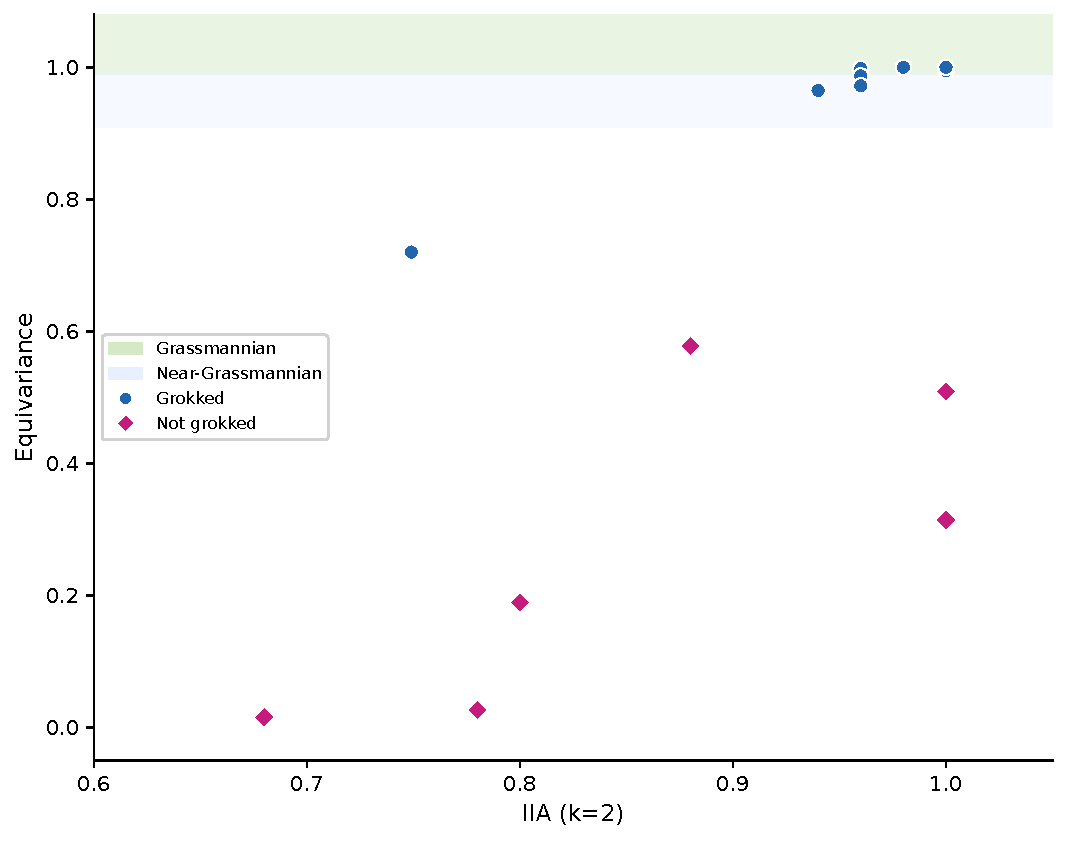
\includegraphics[width=\linewidth]{fig2c_iia_vs_equiv_grokked}
\caption{IIA ($k{=}4$) vs.\ intervention-based equivariance ($k{=}4$)
across 55 operation--prime configurations. Most configurations achieve
IIA $\geq 0.95$, yet equivariance separates grokked operations (blue,
0.04--0.82) from non-grokked (pink, near zero). Unary operations
(gray crosses) are excluded from the main comparison due to degenerate
output structure. Points are jittered horizontally for visibility.}
\label{fig:iia_vs_equiv}
\end{figure}

\subsection{Linear DAS on grokked addition}
\label{sec:linear_das_fails}

Modular addition shows that the Grassmannian assumption can hold at one
subspace dimension and fail at another. We fit DAS across
$k \in \{1, 2, 4, 8, 16, 32\}$ on residual-stream activations from a grokked
model (test accuracy $0.9996$). DAS is near chance at small $k$
($\IIA = 0.006$ at $k = 1$, $0.022$ at $k = 2$, $0.283$ at $k = 4$) and reaches
$\IIA = 1.000$ at $k = 8$ (Table~\ref{tab:ksweep_addition}).

The dimension at which DAS succeeds is informative. The model encodes the
``identity'' of each number $a$ as $(\cos 2\pi f a / p, \sin 2\pi f a / p)$
for key frequencies $f$ \citep{nanda2023progress}. This representation lies on a
circle, which is is a curve rather than a linear subspace, though it lies within the span of
its Fourier components; four key frequencies at two components each span
eight dimensions. DAS succeeds once $k$ reaches that span. The linear constraint
is therefore mismatched to the required dimension at small $k$ rather than
incapable in principle, and reporting DAS at a single small $k$ would
misrepresent it.

This motivates the label-conditional structured VAE approach (\S\ref{sec:vae_results}):
a nonlinear encoder can map the circular representation to a structured
latent space where interchange interventions succeed. On grokked addition, the
label-conditional structured VAE achieves IIA~=~1.0 at $k{=}2$, confirming that the causal
variable exists but is nonlinear.

\begin{table}[t]
\centering
\small
\begin{tabular}{l rrrrrr}
\toprule
& $k{=}1$ & $k{=}2$ & $k{=}4$ & $k{=}8$ & $k{=}16$ & $k{=}32$ \\
\midrule
DAS (linear)            & 0.006 & 0.022 & 0.283 & 1.000 & 1.000 & 1.000 \\
NL-DAS                  & 0.083 & 0.422 & 0.689 & 0.770 & 0.861 & 0.806 \\
\quad $\rho_\text{NL}$  & 0.12  & 0.29  & 0.43  & 0.46  & 0.54  & 0.33 \\
Structured VAE          & 1.000 & 1.000 & 1.000 & 1.000 & 1.000 & 1.000 \\
\quad $\rho_\text{VAE}$ & 1.00  & 1.00  & 1.00  & 1.00  & 0.99  & 1.00 \\
\bottomrule
\end{tabular}
\caption{Grokked modular addition (test accuracy $0.9996$) across subspace
dimension. Linear DAS reaches $\IIA = 1.000$ at $k = 8$, the span of four
Fourier frequencies at two components each. NL-DAS does not exceed $0.861$ at
any dimension tested, and its accuracy and diversity ratio both decline from
$k = 16$ to $k = 32$. Single runs per cell.}
\label{tab:ksweep_addition}
\end{table}

\begin{figure}[t]
\centering
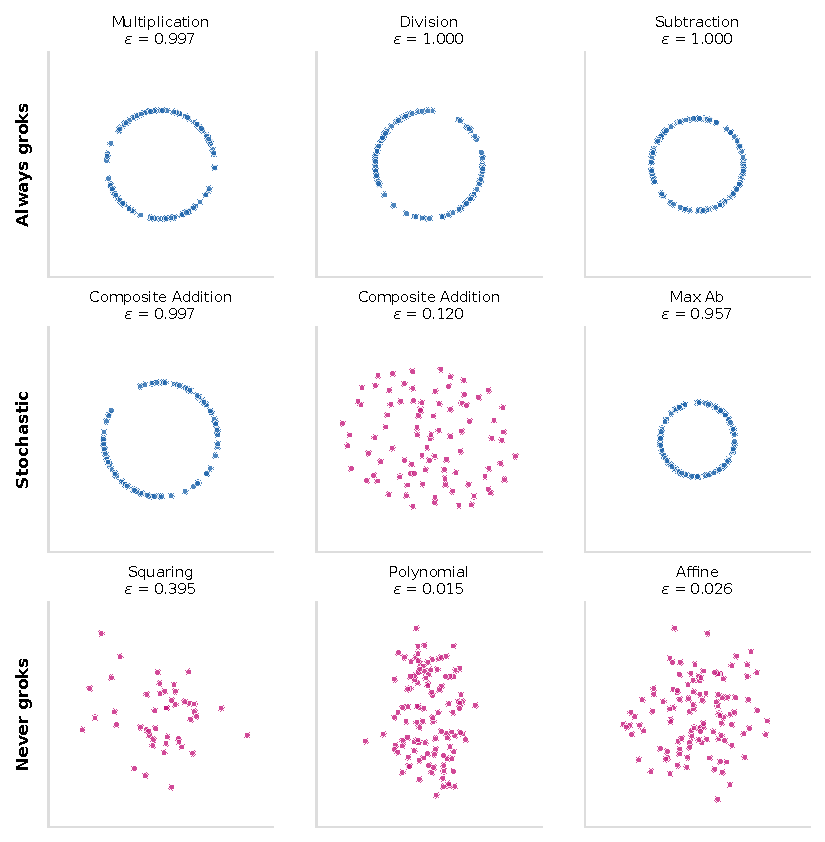
\includegraphics[width=\linewidth]{fig20v2_real_circles_compact}
\caption{DAS 2D projections of label centroids across three grokking
classes. Grokked operations (top two rows, blue) produce centroids
arranged on a circle in the learned subspace, reflecting the group
action's rotational structure. Non-grokked operations (bottom row, pink)
produce unstructured scatter. The stochastic row shows composite
addition under two seeds: one grokked (circular), one not (scattered).}
\label{fig:circle_geometry}
\end{figure}

\subsection{Stochastic grokking}
\label{sec:stochastic}

The multi-modulus sweep reveals that stochastic grokking is a pervasive feature of the boundary region rather than an
anomaly confined to two operations.
A 10-seed stability experiment at $p{=}113$ confirms this directly: composite
addition ($a + b \bmod 91$) groks at exactly 5 of 10 seeds, while power
($a^b \bmod 113$) groks at 0 of 10. The same operation exhibits different grokking behavior across primes: composite
addition groks at $p{=}97$ but not at $p{=}211$ at seed 42. The boundary is
therefore genuinely stochastic rather than a deterministic function of the
operation's algebraic structure.

The multi-modulus data also reveals that operations previously classified as
``never Grassmannian'' were misclassified. Bitwise XOR groks at all four
primes tested, including $p{=}53$ where almost nothing else groks. Sum of
squares groks at three of four primes. These operations were classified as
``never'' based on a single prime ($p{=}113$) where they happened not to
grok---a classification error that the multi-condition sweep corrects.
The lesson is methodological: single-condition classifications of grokking
behavior are unreliable for operations near the boundary.

\begin{figure}[t]
\centering
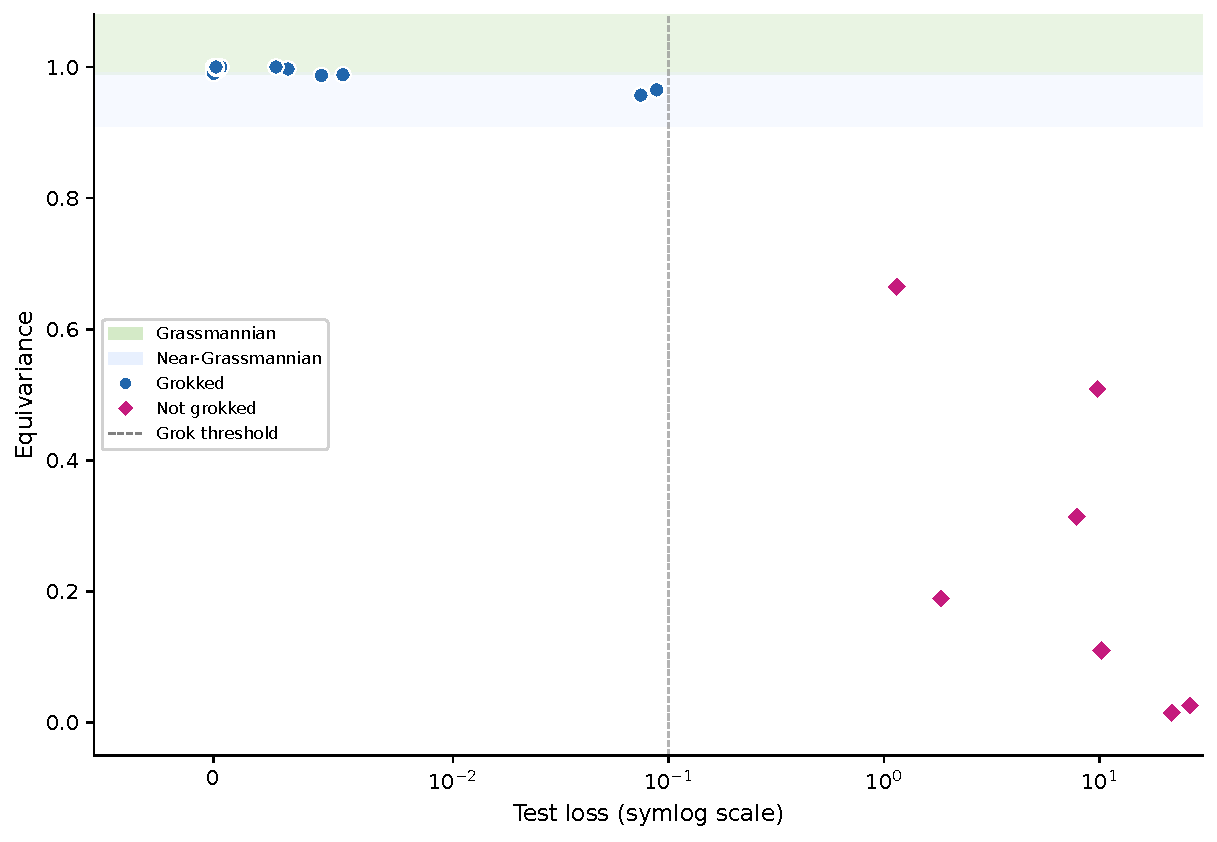
\includegraphics[width=\linewidth]{fig8c_loss_vs_equiv_grokked}
\caption{Test loss vs.\ intervention-based equivariance ($k=4$) across
55 operation--prime configurations.
The dashed line marks the grokking threshold (test loss $= 0.1$).
Grokked operations (blue, left of threshold) achieve equivariance
0.04--0.82; non-grokked operations (pink, right) remain near zero.
Unary operations (gray crosses) are plotted separately: squaring and
cubing show spurious equivariance at some primes due to their
degenerate output structure (see \S\ref{sec:memorization}).
See Appendix~\ref{app:equiv_test} for the equivariance test protocol.}
\label{fig:loss_vs_equiv}
\end{figure}

\subsection{Memorization artifacts}
\label{sec:memorization}

Squaring and cubing reach $\IIA = 0.857$ at $k = 2$ and $\IIA \geq 0.95$ by
$k = 4$ without grokking (test losses $7.8$ and $9.8$ at $p = 113$;
Table~\ref{tab:main_results}). Intervention-based equivariance
exposes the artifact: squaring shows 0\% equivariance at small primes
and a degenerate 50\% at $p = 113, 211$ (likely reflecting output
symmetry rather than genuine structure). The
lesson: \textbf{high IIA with low-$k$ saturation is compatible with a lookup
table}. ``Works for interchange'' and ``is a Grassmannian causal variable'' are
different claims.

\subsection{$k$-sweep profiles and equivariance}

Grassmannian variables saturate at $\IIA \approx 1.0$ by $k = 4$: their causal
structure is inherently 2-dimensional. Non-Grassmannian variables show gradual IIA
growth that may not reach 1.0 even at $k = 32$. Polynomial reaches
$\IIA = 0.72$ at $k = 2$ and requires $k \geq 8$ to approach 0.90.

\begin{figure}[t]
\centering
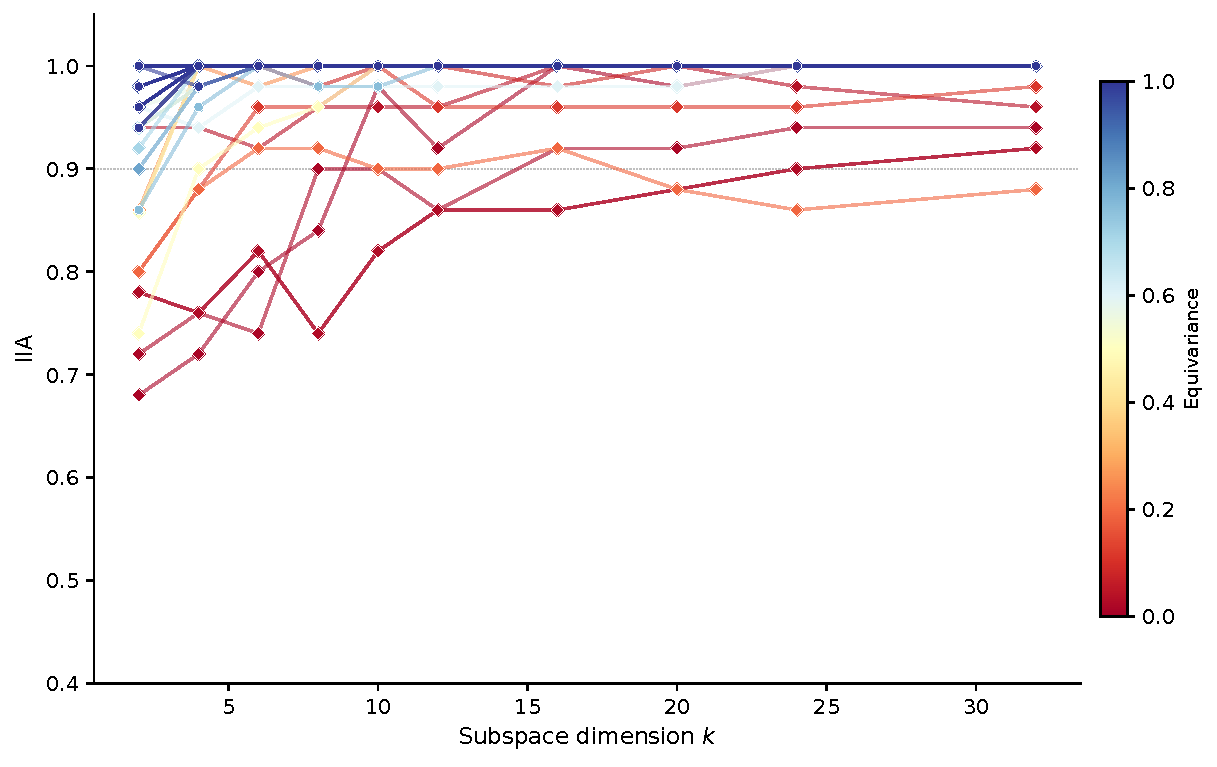
\includegraphics[width=\linewidth]{fig23b_k_sweep_equiv_colored}
\caption{IIA as a function of subspace dimension $k$ for all operations,
colored by equivariance. High-equivariance operations (dark blue)
saturate at $\IIA \approx 1.0$ by $k = 2$--$4$; low-equivariance
operations (red) show gradual growth that plateaus well below 1.0.
The separation between the two regimes is visible at every $k$.}
\label{fig:k_sweep}
\end{figure}

\subsection{Label-conditional structured VAE}
\label{sec:vae_results}

We upgrade the vanilla structured VAE to a \textbf{label-conditional structured VAE}: a
label-conditional structured VAE that partitions the latent space into
$z_\text{causal}$ (supervised, overcomplete) and $z_\text{nuisance}$
(unsupervised). The label-conditional prior follows the identifiable VAE construction of
\citet{khemakhem2020variational}, and the causal/nuisance partition follows
\citet{narayanaswamy2017learning}. The causal latent is expanded $8\times$, so $k$ causal dimensions become $8k$
features.

\paragraph{The $2 \times 2$ ablation.}
Both components---structured prior and expansion---are necessary
(Table~\ref{tab:ablation}). On grokking tasks: (1)~the plain SAE (no
label-conditional prior) achieves IIA~=~1.0 on addition but degrades on harder
operations (multiplication~0.72, quartic sum~0.32); (2)~the label-conditional VAE (structured
prior, no expansion) achieves IIA~$\approx$~0 across all operations;
(3)~\emph{only} the label-conditional structured VAE achieves IIA~=~1.0 uniformly across all
grokked operations and IIA~$\approx$~0 on all non-grokked operations.

\begin{table}[t]
\centering
\small
\setlength{\tabcolsep}{4pt}
\begin{tabular}{@{}l|cc|cc@{}}
\toprule
& \multicolumn{2}{c|}{\textbf{No partition}}
& \multicolumn{2}{c}{\textbf{Causal/nuisance partition}} \\
\textbf{Operation} & Flat & + expansion & Partitioned & \textbf{+ expansion} \\
\midrule
\multicolumn{5}{l}{\textit{Grokked}} \\
Addition       & 0.02 & 1.00 & 0.00 & \textbf{1.00} \\
Multiplication & 0.00 & 0.72 & 0.00 & \textbf{1.00} \\
Quartic sum    & 0.02 & 0.32 & 0.00 & \textbf{1.00} \\
IOI (GPT-2)    & 0.56 & 0.83 & 0.95 & \textbf{0.98} \\
\midrule
\multicolumn{5}{l}{\textit{Non-grokked (correct answer: $\approx 0$)}} \\
Mixed product  & 0.03 & 0.01 & 0.01 & 0.04 \\
Squaring       & 0.00 & 0.00 & 0.00 & 0.00 \\
\bottomrule
\end{tabular}
\caption{$2{\times}2$ ablation: IIA at $k{=}2$. All four models use the
label-conditional prior; the columns vary the causal/nuisance partition and the
eightfold expansion of the causal latent. The expansion carries modular addition
on its own ($1.00$) and degrades on harder operations (multiplication $0.72$,
quartic sum $0.32$). The partition without the expansion reaches $0.00$ on every
grokked operation. Combining them reaches $1.00$ on all grokked operations and
$\leq 0.04$ on all non-grokked ones. Single runs per cell.}
\label{tab:ablation}
\end{table}

\paragraph{Reconstruction MSE as a falsifiability criterion.}
For non-grokked operations, reconstruction MSE is $11$--$24$; for grokked
operations, $0.6$--$1.2$.  High MSE with near-zero IIA means the model has
\emph{no structured causal variable to recover}---not that the method
failed.  This diagnostic is unavailable for NL-DAS, which returns IIA $=
0.6$--$0.8$ on non-grokked operations (false positives) because it has no
reconstruction constraint.

\paragraph{End-to-end intervention training.}
For language model tasks where the causal structure is more complex, we add an
\textbf{end-to-end (E2E) intervention CE loss}: after swapping $z_\text{causal}$
and decoding, we run the intervened activation through the remaining layers and
compute $-\log p(y_s \mid h')$. This differentiable objective directly
optimizes for intervention success. It is \emph{added} to the ELBO rather than
substituted for it, so the generative terms stay active throughout training. The
method therefore optimizes the same objective as NL-DAS subject to constraints
NL-DAS lacks, which makes the comparison between the two controlled: the
objective is held fixed and only the constraint set varies. Training proceeds in two phases: 200 epochs of reconstruction +
classification warmup, followed by E2E intervention training with an additive
intervention $h' = h_b + \text{dec}(z_\text{swap}) - \text{dec}(z_\text{orig})$
that cancels reconstruction error.

\paragraph{Validation on GPT-2 language tasks.}
The label-conditional structured VAE was developed to recover nonlinear causal variables in
grokking models. One concern is whether it overfits to the specific
geometry of modular arithmetic. To test generalization, we evaluate on six
tasks from the MIB benchmark \citep{mueller2025mib} at layer~8 of GPT-2-small,
where DAS is the established baseline (Table~\ref{tab:nlp_results}).

\begin{table}[t]
\centering
\small
\setlength{\tabcolsep}{4pt}
\begin{tabular}{lcccc}
\toprule
\textbf{Task} & \textbf{DAS} & \textbf{DAS (strict)} & \textbf{E2E} & \textbf{E2E (strict)} \\
\midrule
IOI            & 0.19 & 0.19 & \textbf{1.00} & \textbf{1.00} \\
Gender bias    & 0.62 & 0.52 & \textbf{1.00} & \textbf{1.00} \\
Greater-than   & 0.93 & 0.28 & \textbf{1.00} & \textbf{1.00} \\
SVA            & 0.92 & 0.00 & \textbf{1.00} & \textbf{1.00} \\
Hypernymy      & 0.07 & 0.02 & \textbf{0.97} & \textbf{0.90} \\
Capitals$^\dagger$ & 0.12 & 0.00 & \textbf{0.51} & \textbf{0.26} \\
\bottomrule
\end{tabular}
\caption{Standard and strict IIA at $k{=}1$ on six GPT-2 language tasks
(layer~8, additive intervention). label-conditional structured VAE with E2E training
dominates DAS on all six tasks. $^\dagger$Capitals has 182 classes with
only 190 examples ($\approx$1 per class), limiting classifier training.}
\label{tab:nlp_results}
\end{table}

The label-conditional structured VAE with E2E training matches or exceeds DAS on all six
GPT-2 tasks at $k{=}1$, confirming that the method is not specific to
grokking geometry. On five of six tasks, E2E achieves strict IIA $\geq 0.90$;
on IOI, gender bias, greater-than, and SVA it reaches 1.00. The sole
exception is capitals, where the dataset contains 182 classes with only 190
examples, limiting classifier training. On hypernymy, E2E achieves
IIA~=~0.97 at $k{=}1$---$14\times$ better than DAS (0.07)---and DAS's strict
IIA on SVA is exactly 0.00 despite standard IIA of 0.92, revealing that DAS
shifts probability mass toward the correct token without ever making it the
argmax. These results serve as a sanity check: the label-conditional structured VAE is a
strict generalization of DAS (matching it where linear structure suffices,
exceeding it where nonlinear structure is needed), not a special-case method.

\paragraph{Capacity comparison.}
The methods differ substantially in parameter count
(Table~\ref{tab:params}). DAS learns only the rotation $Q$; Structured VAE adds
an encoder-decoder with reconstruction constraints; NL-DAS adds an MLP
featurizer without constraints. Structured VAE (E2E) uses the same architecture
as Structured VAE but trains with intervention loss end-to-end. The Structured VAE's
additional capacity is spent on reconstruction and regularization, not
on memorizing intervention pairs---as the diversity ratio confirms.

\begin{table}[t]
\centering
\small
\begin{tabular}{lrl}
\toprule
Method & Parameters & Constraints \\
\midrule
DAS         & 768     & None (linear rotation) \\
NL-DAS      & $\sim$787K  & None (end-to-end IIA only) \\
Structured VAE      & $\sim$414K  & ELBO + KL + causal/nuisance split \\
Structured VAE (E2E)  & $\sim$414K  & ELBO + KL + split + IIA \\
\bottomrule
\end{tabular}
\caption{Parameter counts at $k{=}1$ on GPT-2 ($d = 768$, hidden $= 512$,
  latent $= 16$). NL-DAS has $1.9\times$ the parameters of Structured VAE with
  zero structural constraints, enabling the lookup-table failure mode.}
\label{tab:params}
\end{table}

On IOI \citep{wang2022interpretability}, NL-DAS achieves IIA~$= 1.00$,
but the diversity ratio $\rho \approx 0.05$ (vs.\ $\rho \approx 0.89$ for the
label-conditional VAE) exposes it as vacuous (Table~\ref{tab:nldas_vacuous}).

\subsection{Unconstrained nonlinear DAS}
\label{sec:nldas_vacuous}

One response to DAS's linearity constraint is to prepend an MLP
featurizer: learn a nonlinear coordinate system in which the causal variable
\emph{becomes} linear, then apply standard DAS. This approach---which we call
NL-DAS (\S\ref{sec:nldas})---achieves IIA~=~1.000 on IOI at $k = 1$, compared
to DAS's 0.183. The diversity ratio qualifies that improvement.

\paragraph{The lookup-table failure mode.}
NL-DAS is trained end-to-end on interchange loss with no reconstruction
constraint. The encoder $f$ and decoder $g$ need not be approximate inverses,
and the training objective provides no incentive for them to be. This creates a
degenerate solution: $f$ maps every activation to a space where the first
coordinate encodes the class label and the remaining coordinates are arbitrary;
$g$ ignores the base-specific content entirely and produces a ``canonical
activation for class $y_s$'' regardless of which base input was used.

The intervention diversity ratio (\S\ref{sec:faithfulness_metrics}) exposes this
failure. Table~\ref{tab:nldas_vacuous} reports results for IOI and two
grokking operations (addition, multiplication mod 113) across $k \in \{1, 2, 4\}$;
squaring did not grok within 80{,}000 epochs.

\begin{table}[t]
\centering
\small
\setlength{\tabcolsep}{3pt}
\begin{tabular}{lc rrrr rr}
\toprule
Task & $k$ & DAS & NL-DAS & NL-DAS+r & VAE & $\rho_\text{NL}$ & $\rho_\text{VAE}$ \\
\midrule
IOI & 1 & 0.183 & 1.000 & 0.867 & 1.000 & 0.05 & 0.83 \\
IOI & 2 & 0.322 & 1.000 & 0.700 & 0.989 & 0.05 & 0.89 \\
IOI & 4 & 0.572 & 1.000 & 0.811 & 0.989 & 0.05 & 0.92 \\
\midrule
Addition & 1 & 0.006 & 0.083 & 0.028 & 1.000 & 0.12 & 1.00 \\
Addition & 2 & 0.022 & 0.422 & 0.039 & 1.000 & 0.29 & 1.00 \\
Addition & 4 & 0.283 & 0.689 & 0.033 & 1.000 & 0.43 & 1.00 \\
\midrule
Mult.\ & 1 & 0.028 & 0.239 & 0.028 & 1.000 & 0.65 & 1.00 \\
Mult.\ & 2 & 0.072 & 0.544 & 0.111 & 1.000 & 1.00 & 1.00 \\
Mult.\ & 4 & 0.283 & 0.933 & 0.372 & 1.000 & 1.12 & 0.99 \\
\midrule
Squaring & $\dagger$ & \multicolumn{6}{c}{\emph{did not grok ($\text{acc} = 0.00$)}} \\
\bottomrule
\end{tabular}
\caption{NL-DAS achieves high IIA by learning degenerate encoder-decoders.
  The VAE column reports label-conditional structured VAE results.
  $\rho$ is the intervention diversity ratio (Eq.~\ref{eq:diversity_ratio});
  NL-DAS+r adds a reconstruction penalty ($\lambda_\text{recon} = 0.1$).
  $\dagger$Squaring ($x^2 \bmod 113$) failed to grok within 80{,}000 epochs
  at all tested $k$.
  Controls (random labels, reconstruction-only, untrained probe, unconstrained
  plain VAE) are reported in \S\ref{sec:controls} against per-task chance
  rather than a single bound, since chance accuracy varies with class count.}
\label{tab:nldas_vacuous}
\end{table}

Two lines of evidence support this:

\begin{enumerate}[leftmargin=*]
\item \textbf{Controls rule out the structured VAE cheating.} Random-label
  supervision, reconstruction-only training ($\alpha = 0$), an untrained probe,
  and an unconstrained plain VAE with no causal/nuisance split all fail, each at
  or near the chance accuracy for its task (\S\ref{sec:controls}). The structured
  VAE's success requires correct supervision \emph{and} the
  causal-nuisance partition. NL-DAS lacks the reconstruction constraint
  that prevents degenerate solutions; without inductive biases, unsupervised
  disentanglement is impossible \citep{locatello2019challenging}.

\item \textbf{The structured prior and reconstruction constraint are
  necessary, not optional.} The ELBO forces the decoder to produce
  activations close to the original, the KL regularization prevents
  encoder collapse, and the causal-nuisance partition ensures that
  base-specific information is preserved in $z_\text{nuisance}$.
  NL-DAS has none of these constraints.
\end{enumerate}

\paragraph{Why the VAE is not vacuous.}
The structured VAE's ELBO provides three constraints that prevent the
lookup-table failure mode: (1)~the reconstruction loss forces the decoder to
produce activations close to the original, not class-specific templates;
(2)~the KL regularization prevents the encoder from collapsing the latent space
to a few discrete points; and (3)~the causal-nuisance partition ensures that
$z_\text{nuisance}$ absorbs base-specific information, so the decoder must use
it. Together, these constraints mean that swapping $z_\text{causal}$ while
preserving $z_\text{nuisance}$ genuinely modifies only the causal component.

\paragraph{Implications.}
These results suggest that nonlinear methods for causal abstraction should be
evaluated with intervention faithfulness metrics alongside IIA. The NL-DAS failure mode is not specific to
our architecture---it is an instance of the non-linear representation dilemma
established by \citet{sutter2025nonlinear}, who prove that without structural
constraints an unconstrained nonlinear alignment map can match any network to any
algorithm at perfect IIA, and who demonstrate it directly by reaching 100\% IIA
on randomly initialised language models. We reproduce their result in our setting
rather than establishing it, and ask what a constrained map does under the same
test: the ELBO's
reconstruction and regularization terms exclude the degenerate solutions we
observe. We do not establish that they restore identifiability.
Prior work proposing neural network featurizers for causal abstraction
\citep{geiger2024causal} should be re-evaluated with diversity ratio and
reconstruction checks.

\subsection{Controls}
\label{sec:controls}

Four ablations test whether the label-conditional structured VAE succeeds for the
stated reasons: random-label supervision, reconstruction-only training
($\alpha = 0$), an untrained probe, and an unconstrained plain VAE with no
causal/nuisance partition. Each is compared against the accuracy of a random
subspace on the same task, because chance accuracy varies with class count and
task structure rather than sitting at zero.

\begin{table}[t]
\centering
\small
\setlength{\tabcolsep}{5pt}
\begin{tabular}{l r rrrr}
\toprule
Task & Random subspace & Random labels & Recon.\ only & Untrained & Plain VAE \\
\midrule
IOI                  & 0.000 & 0.002 & 0.000 & 0.000 & 0.000 \\
Hypernymy            & 0.000 & 0.000 & 0.000 & 0.000 & 0.000 \\
Addition ($p{=}113$) & 0.000 & 0.000 & 0.000 & 0.000 & 0.000 \\
Capitals             & 0.105 & 0.105 & 0.105 & 0.105 & 0.105 \\
Gender bias          & 0.274 & 0.230 & 0.277 & 0.277 & 0.277 \\
Greater-than         & 0.450 & 0.453 & 0.450 & 0.450 & 0.450 \\
Subject--verb agr.\  & 0.482 & 0.482 & 0.482 & 0.482 & 0.522 \\
\bottomrule
\end{tabular}
\caption{Controls against the random-subspace floor at $k = 1$. Every control
matches its task's floor to within $0.04$. The floor itself ranges from $0.000$
to $0.482$, so a single numeric bound across tasks would be uninformative: the
same value that indicates failure on IOI would indicate nothing on subject--verb
agreement. Success on these tasks therefore requires correct supervision and the
causal/nuisance partition, neither of which any control retains.}
\label{tab:controls_main}
\end{table}

Table~\ref{tab:controls_main} reports the comparison. Every control is
indistinguishable from a random subspace, which is the relevant statement: the
label-conditional structured VAE's accuracy does not survive removing the label
supervision, the reconstruction term, training, or the latent partition.

\subsection{Random-network control}
\label{sec:randomnet}

The sharpest form of \citet{sutter2025nonlinear}'s result is empirical rather
than theoretical: their alignment maps reach 100\% interchange accuracy on
\emph{randomly initialised} language models, networks that cannot perform the
task at all. High accuracy obtained that way carries no information about the
network, which is what makes the test decisive. The test is theirs. They apply it
to unconstrained maps; we apply it to a constrained one, which they do not
examine.

We run both arms under identical settings, varying only the base model's weights.
On the random arm the counterfactual target is set by the task rather than by the
model's own outputs, since a random model is correct on nothing.

\begin{table}[t]
\centering
\small
\setlength{\tabcolsep}{5pt}
\begin{tabular}{l rr rr}
\toprule
& \multicolumn{2}{c}{Pretrained GPT-2} & \multicolumn{2}{c}{Randomly initialised} \\
\cmidrule(lr){2-3}\cmidrule(lr){4-5}
Method & IIA & $\rho_\text{within}$ & IIA & $\rho_\text{within}$ \\
\midrule
DAS (linear)            & 0.194 & 1.391 & 0.000 & 0.892 \\
NL-DAS                  & 1.000 & 0.079 & \textbf{0.989} & 1.068 \\
NL-DAS + reconstruction & 0.944 & 2.249 & 0.806 & 1.532 \\
Structured VAE          & 1.000 & 0.561 & \textbf{0.000} & 0.629 \\
\bottomrule
\end{tabular}
\caption{Indirect object identification at $k = 1$, 5000 NL-DAS steps, on
pretrained GPT-2 and on the same architecture with every parameter
re-initialised. The random-network test is \citet{sutter2025nonlinear}'s; the
constrained map is what we add to it. Replicated at 2000 steps across three
seeds, where NL-DAS reaches $0.944$--$0.961$ on the random arm and the structured
VAE reaches $0.000$ on all three.}
\label{tab:randomnet}
\end{table}

Destroying the network costs the unconstrained map $0.011$
(Table~\ref{tab:randomnet}). NL-DAS reaches $\IIA = 0.989$ on a network with no
causal structure, reproducing \citeauthor{sutter2025nonlinear}'s finding in our
setting. The constrained map reaches $0.000$. The separation held in all five
runs we conducted, across three seeds and two optimisation budgets.

This is also the answer to an objection the method invites. The structured VAE
supervises its causal latent with the task label, so a reader may reasonably ask
whether interchange succeeds by routing the answer through that latent rather
than through the model's computation, which would be the same lookup-table
failure we attribute to NL-DAS. A random network contains no causal structure, so
any accuracy above chance there is leakage. The method scores zero. The decision
rule was fixed before the run: had it exceeded $0.30$, the claim would have been
withdrawn.

\subsection{Limits of the diversity ratio}
\label{sec:rho_fails}

The diversity ratio is ours, and it does not survive this test.

Read the $\rho_\text{within}$ column of Table~\ref{tab:randomnet} against the
interpretation we gave it in \S\ref{sec:faithfulness_metrics}. NL-DAS scores $0.079$ on
pretrained GPT-2, which that interpretation calls a collapsed lookup table, and
$1.068$ on the random network, which it calls faithful. The metric clears the
case with no causal structure and flags the case where structure exists. It
inverts.

Optimisation budget explains the inversion. NL-DAS random-arm accuracy rises with
steps ($0.906$ at 2000, $0.989$ at 5000), and its $\rho_\text{within}$ falls
toward 1 over the same range ($1.7$--$2.2$ across seeds at 2000, $1.068$ at
5000). Under-optimised, the map forces the output through visible distortion.
Given more steps it finds a solution that is both near-perfect and metrically
indistinguishable from a faithful intervention. A vacuous map can look faithful
once it has been trained long enough.

We therefore report $\rho$ as a secondary signal and not as a sufficient test.
This is the reason \citeauthor{sutter2025nonlinear}'s control is load-bearing
rather than a redundant check: if an auxiliary faithfulness metric were
sufficient, one could measure $\rho$ on the pretrained arm and stop. Ours is not
sufficient, so the random-network test carries the claim.

One observation remains unexplained. NL-DAS with a reconstruction penalty reaches
$\rho_\text{within} = 2.249$ on the \emph{pretrained} arm at $\IIA = 0.944$, so
high dispersion accompanies high accuracy on real structure as well. We have no
account of it.

\subsection{Cross-distribution generalization}
\label{sec:cross_distribution}

The standard IOI evaluation draws train and test data from the same
distribution of names and templates. This leaves open whether methods
generalize across distributional shifts or merely memorize the training
distribution. We evaluate two held-out splits: \emph{disjoint names}
(test entities never appear in training) and \emph{disjoint templates}
(test sentence structures never appear in training).
Table~\ref{tab:cross_dist} reports IIA and diversity ratio $\rho$ at $k{=}1$.

\begin{table}[t]
\centering
\small
\setlength{\tabcolsep}{3pt}
\begin{tabular}{l rr rr rr}
\toprule
& \multicolumn{2}{c}{Standard} & \multicolumn{2}{c}{Disjoint names} & \multicolumn{2}{c}{Disjoint templates} \\
\cmidrule(lr){2-3}\cmidrule(lr){4-5}\cmidrule(lr){6-7}
Method & IIA & $\rho$ & IIA & $\rho$ & IIA & $\rho$ \\
\midrule
DAS           & 0.183 & ---  & 0.035 & ---  & 0.166 & ---  \\
NL-DAS        & 1.000 & 0.05 & 1.000 & 0.05 & 0.537 & 0.05 \\
Structured VAE        & 1.000 & 0.83 & 0.001 & 0.78 & 0.963 & 0.51 \\
Structured VAE (E2E)    & 1.000 & 0.83 & 0.001 & 0.80 & \textbf{0.993} & 0.53 \\
\bottomrule
\end{tabular}
\caption{Cross-distribution generalization on IOI at $k{=}1$.
  NL-DAS maintains IIA~$= 1.0$ on disjoint names because its
  lookup table ignores input identity ($\rho = 0.05$).
  Structured VAE correctly reports IIA~$\approx 0$ on disjoint names---the
  causal variable is token-specific and does not transfer between
  entity sets.
  On disjoint templates, Structured VAE (E2E) achieves IIA~$= 0.993$ with
  $\rho = 0.53$, confirming genuine generalization across surface
  forms.}
\label{tab:cross_dist}
\end{table}

Plotting accuracy against diversity separates the two regimes directly
(Figure~\ref{fig:iia_vs_diversity}).

\paragraph{Honest failure vs.\ vacuous success.}
The disjoint-names split creates a revealing separation. NL-DAS
reports IIA~$= 1.0$ because its degenerate encoder maps all
activations to class-conditional templates regardless of which
entity tokens appear---the lookup table transfers perfectly because it
never encoded entity identity in the first place. The label-conditional VAE
reports IIA~$\approx 0$ because its reconstruction constraint forces
the encoder to preserve entity-specific activation structure; swapping
the causal component from one entity set into a base from a different
set produces incoherent reconstructions. This is the \emph{correct}
answer: the IOI causal variable (indirect object identity) is
inherently token-specific, and interventions between entity sets
\emph{should} fail. A method that reports success on this split is
vacuous by construction.

\begin{figure}[t]
\centering
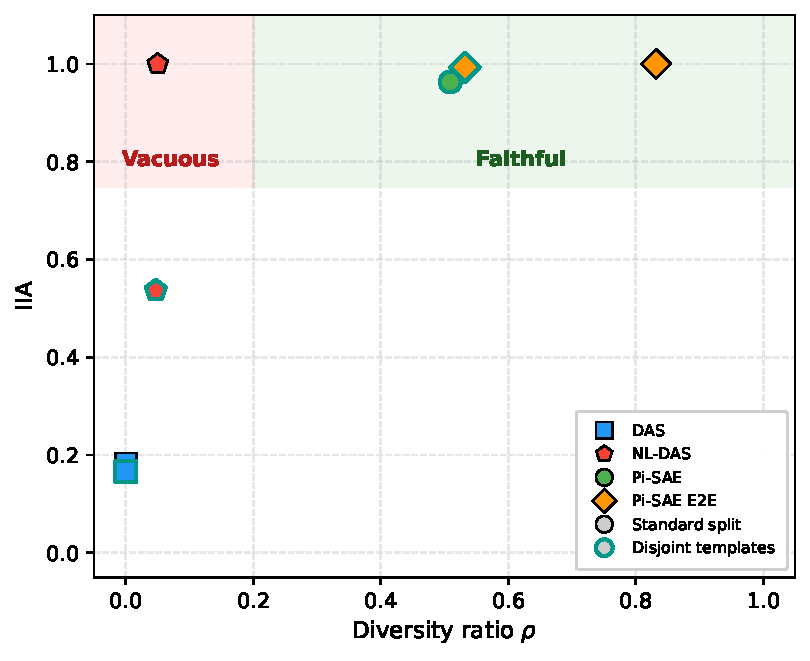
\includegraphics[width=0.85\linewidth]{fig_iia_vs_diversity}
\caption{IIA vs.\ diversity ratio $\rho$ across methods and distribution
splits (IOI, $k{=}1$). Vacuous methods (top-left, red shading) achieve
high IIA with $\rho \approx 0$: the encoder-decoder collapses to a
lookup table. Genuine methods (top-right, green shading) maintain high
$\rho$, confirming input-specific interventions. NL-DAS occupies the
vacuous region across all splits. Structured VAE (E2E) on disjoint templates
($\IIA = 0.993$, $\rho = 0.53$) confirms genuine cross-distribution
generalization. Edge color indicates split: black = standard, purple =
disjoint names, teal = disjoint templates.}
\label{fig:iia_vs_diversity}
\end{figure}

On disjoint templates, the situation reverses: the causal variable
transfers across sentence structures because the underlying
computation (attending to the indirect object position) is
template-invariant. Structured VAE (E2E) achieves IIA~$= 0.993$ with
$\rho = 0.53$, confirming that the learned subspace captures
genuine causal structure. NL-DAS drops to IIA~$= 0.537$---its
template-specific lookup table partially fails when sentence
structure changes, yet maintains $\rho = 0.05$, indicating the
encoder-decoder remains degenerate.

\subsection{Group action and linearity}

Affine ($2a + 3b + 5 \bmod 113$) is a linear function that fails to produce a
Grassmannian variable. Under an additive shift $a \mapsto a + g$ the output
shifts by $2g$ rather than $g$, so the operation is not a group action even
though it is linear. Intervention-based equivariance is 0\% across all four
primes tested. Linearity of the operation and linearity of the causal variable
are therefore separate properties, and the second is the one DAS assumes.

Two boundary cases fill in the picture. Cubic sum ($a^3 + b^3 \bmod 113$)
achieves high equivariance while cubing alone shows 0\% (intervention-based,
$k{=}4$, $p{=}113$), so the binary structure supplies additive symmetry that the
unary operation lacks. Max ($\max(a,b) \bmod p$) is piecewise equivariant,
reaching 15\% at $p{=}113$ and 29\% at $p{=}53$ ($k{=}4$): when the argmax is
stable under the shift it behaves like a shifted identity, and the partial
equivariance reflects that conditional structure.

\section{Mechanism}
\label{sec:mechanism}

The atlas (\S\ref{sec:results}) established \emph{what}: causal structure
emerges through grokking, with the boundary depending on operation, dataset
size, and model depth. This section asks \emph{how} and \emph{why}.

\paragraph{Summary of mechanistic findings (full details in
Appendix~\ref{app:mechanistic}).}
Architecture ablations show that nonlinearity is necessary for grokking
(linear DMF never generalizes despite spectral compression) while attention
is not (DMF + ReLU groks $18\times$ faster than the full transformer;
Table~\ref{tab:grokking_speed}). Fine-grained trajectory analysis reveals
that generalization precedes Fourier crystallization by $\sim$1{,}000 epochs
(Table~\ref{tab:fourier_lag}): the gradient discovers Fourier structure
$\sim$10{,}000 epochs before the weights do, as measured by the AGOP
(Table~\ref{tab:agop}). During grokking, the feedforward product matrix
$W_\text{in} W_\text{out}$ undergoes $5.3\times$ rank collapse (effective
rank 48 $\to$ 9), but compression alone is insufficient---the compressed
subspace must also acquire equivariance under the operation's symmetry group
(Figure~\ref{fig:trajectory}).

The two findings most relevant to the Grassmannian interpretation---that
the causal variable is readable from weight-space without optimization,
and that the causal subspace is degenerate---are presented below.

\subsection{Weight-space SVD}
\label{sec:svd_vs_das}

If grokking compresses the solution into a low-rank subspace, can we read the
causal variable directly from the weight matrices without fitting DAS? We
compare SVD of the feedforward product matrix against DAS fitted to
activations, measuring IIA for both.

\begin{table}[t]
\centering
\small
\begin{tabular}{llrl}
\toprule
Method & Site & Best $k$ & IIA \\
\midrule
SVD(FF) & attn\_out & 32 & \textbf{0.999} \\
DAS     & attn\_out & 8  & 0.150 \\
DAS     & mlp\_out  & 8  & 0.631 \\
SVD(FF) & mlp\_out  & 64 & 0.444 \\
\bottomrule
\end{tabular}
\caption{SVD of the feedforward product matrix vs.\ DAS on a grokked
multiplication model. At the attn\_out site, SVD achieves IIA = 0.999
\emph{with no optimization} (DAS: 0.150 after 200 gradient steps).
The Grassmannian distance between SVD and DAS subspaces is
1.5--8.2~radians (near-orthogonal).}
\label{tab:svd_vs_das}
\end{table}

Table~\ref{tab:svd_vs_das} reports the comparison. At the attention output
site, SVD(FF) achieves $\IIA = 0.999$ at $k = 32$
with \emph{zero optimization}---no gradient steps, no interchange
training---while DAS achieves only 0.150 at $k = 8$ after 200 gradient
steps. \textbf{Caveat}: the comparison is not dimension-matched. SVD
requires $4\times$ the subspace dimension, reflecting that the top singular
vectors of $W_\text{FF}$ include directions relevant to the causal variable
but also spectral directions that are not causally active. A fair evaluation
requires comparing both methods at matched $k$ values, which we leave for
future work. The current result shows that the causal variable is
\emph{readable} from weight-space structure without optimization, not that
SVD is a superior method to DAS.

The Grassmannian distance between the SVD and DAS subspaces ranges from
1.5 to 8.2 radians---they are near-orthogonal. This is consistent with
the subspace degeneracy finding (\S\ref{sec:gauge_freedom}): many different
subspaces carry the same causal information. The SVD subspace is one
valid parameterization; the DAS subspace is another. Neither is
``correct''---both are equivalent points in the orbit of the gauge
group acting on $\Gr(k,d)$.

The site dependence is notable: SVD(FF) is most informative at attn\_out
(where the attention output has been computed) but weaker at mlp\_out
(where the MLP has further mixed the representation). DAS shows the
opposite pattern, achieving 0.631 at mlp\_out. This suggests that
weight-space and activation-space methods have complementary strengths:
SVD captures the structural potential of the weight matrices, while DAS
captures the functional use of that structure under the data distribution.

\subsection{Subspace degeneracy}
\label{sec:gauge_freedom}

If grokking produces a specific causal subspace, we might expect different
random seeds to converge to the \emph{same} point on $\Gr(k,d)$. They do
not. Ten seeds of modular multiplication all grok successfully ($\IIA$
0.94--1.00), but the recovered DAS subspaces are nearly orthogonal: pairwise
overlap $\approx 0.008$, where random $k$-dimensional subspaces of
$\R^{128}$ would have expected overlap $k/d = 0.016$. The grokked subspaces
are \emph{less} aligned than chance---consistent with the null distribution
of random subspaces on $\Gr(2, 128)$, where pairwise geodesic distances
concentrate around $\pi/2 \cdot \sqrt{k} \approx 2.22$ radians (the
observed range is $[1.93, 2.19]$).

\paragraph{The basin of attraction is enormous.}
Perturbing the DAS subspace by rotating it 1+ radians on $\Gr(k,d)$
barely drops IIA. The causal variable is not a fragile low-dimensional
needle in a high-dimensional haystack---it is a robust feature of the
representation that can be read out from exponentially many subspaces.

The same near-orthogonality holds across operations as well as across seeds
(Figure~\ref{fig:principal_angles}).

\paragraph{Spectral graph structure.}
Computing the pairwise Grassmannian distance between all 10 seeds'
subspaces yields a nearly uniform distance matrix:
$d_{\Gr} \in [1.93, 2.19]$. The subspaces are equidistant from each other,
forming a ``spectral simplex'' on the Grassmannian rather than clustering
around a preferred direction.

\begin{figure}[t]
\centering
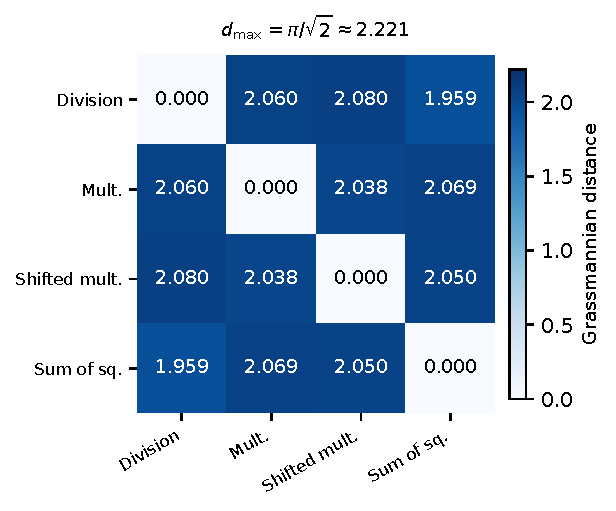
\includegraphics[width=0.7\linewidth]{fig4_principal_angles}
\caption{Pairwise Grassmannian distances between DAS subspaces fitted
to four grokked operations. All distances cluster near
$d_\mathrm{max} = \pi/\sqrt{2} \approx 2.22$ radians, indicating
near-orthogonal subspaces. Each operation learns a valid causal
variable, but these variables occupy different regions of
$\Gr(2, 128)$.}
\label{fig:principal_angles}
\end{figure}

This finding has a concrete implication for mechanistic interpretability:
the identity of a recovered subspace carries less information than its
equivalence class under the symmetry acting on $\Gr(k,d)$.
All 10 seeds converge to the same orbit under the symmetry group acting on
$\Gr(k,d)$---they agree on the gauge-invariant causal information, even
though they disagree on which representative subspace carries it.
Two analyses of the same model at different random seeds find orthogonal DAS
solutions, but both solutions support equally valid interventions. The
model's computation defines a large equivalence class on $\Gr(k,d)$: many
subspaces carry the same causal information, analogous to the rotational
degeneracy in attention circuits where $W_Q \to W_Q R$,
$W_K \to W_K R$ leaves $W_Q W_K^\top$ invariant. The relevant object is
not a point on $\Gr(k,d)$ but an orbit, and functional diagnostics
(equivariance, IIA) are orbit-invariant while structural diagnostics
(subspace identity) are not.

\section{Discussion}
\label{sec:discussion}

\subsection{Evaluation diagnostics}
\label{sec:diagnostics}

The evaluations we report are not ordered by strength. Each catches a different
way a causal-variable claim can go wrong, and a method can pass one while failing
another: linear DAS satisfies faithfulness by construction yet reached
$\IIA = 0.006$ at $k = 1$ on grokked addition, while NL-DAS reached
$\IIA = 1.000$ on IOI with $\rho = 0.05$. Table~\ref{tab:diagnostics} summarises
what each measurement caught in our experiments.

\begin{table}[t]
\centering
\small
\setlength{\tabcolsep}{4pt}
\begin{tabular}{@{}p{3.1cm}p{4.6cm}p{5.6cm}@{}}
\toprule
Diagnostic & Failure mode it catches & Instance in this paper \\
\midrule
Interchange accuracy &
Method cannot support interchange at all &
Linear DAS, $\IIA = 0.006$ at $k{=}1$ on grokked addition \\
\addlinespace
Diversity ratio $\rho$; reconstruction MSE &
Decoder ignores the base input and emits a per-label template &
NL-DAS on IOI, $\IIA = 1.000$ at $\rho = 0.05$ \\
\addlinespace
Distributional metrics (KL, JS) &
Top-1 flips while the rest of the distribution is distorted &
DAS on subject--verb agreement, $0.92$ standard against $0.00$ strict \\
\addlinespace
Equivariance; cross-distribution transfer &
High accuracy from memorisation or distributional artifacts &
Squaring, $\IIA = 0.857$ at $k{=}2$ without grokking \\
\bottomrule
\end{tabular}
\caption{Each diagnostic detects a distinct failure mode. They are independent
rather than ordered: passing one does not imply passing another. We do not claim
the set is exhaustive.}
\label{tab:diagnostics}
\end{table}

Linear DAS is faithful by construction, since the orthogonal projection modifies
only the subspace component, and can still fail on accuracy when the causal
variable needs more dimensions than the chosen $k$. Unconstrained nonlinear maps
reach high accuracy readily and fail on faithfulness. The label-conditional
structured VAE passed both in our experiments, which we attribute to the ELBO's
reconstruction and regularisation terms excluding the degenerate solutions.

\subsection{Grokking and causal structure}

The multi-condition atlas shows that grokking is the process by which a model's
internal representation transitions from an unstructured memorization encoding to
a structured causal encoding. The stochastic grokking discovery---where the same
operation groks at one prime or seed but not another---provides the cleanest
evidence for this claim, because it controls for everything except the
generalization transition itself. The multi-modulus sweep strengthens this
evidence: an operation can be ``never Grassmannian'' at $p{=}53$ and ``always
Grassmannian'' at $p{=}211$, with the transition governed by whether sufficient
data exists to drive grokking. For operations with linear algebraic structure,
the resulting encoding lives on $\Gr(k,d)$ and DAS recovers it. For operations
with nonlinear structure, the encoding lives on a curved manifold and requires
nonlinear methods to access.

The mechanism section (\S\ref{sec:mechanism}) reveals that this transition
involves three dissociable processes: spectral compression (effective rank
$48 \to 9$), Fourier crystallization (which \emph{lags} generalization by
$\sim$1{,}000 epochs), and the selection of one among exponentially many
equivalent causal subspaces (subspace degeneracy). The AGOP analysis
(\S\ref{app:fourier_trajectory}) provides a concrete timeline: the gradient
discovers Fourier structure $\sim$10{,}000 epochs before the weights do,
and the actual phase transition is marked by a temporary \emph{dip} in
gradient-space Fourier alignment before crystallization.
% TODO: The effective rank drop (48->9) reported here for the atlas is mirrored
% in Phase C stochastic grokker trajectories (29->17, 26->21) and is temporally
% locked to the grokking epoch. Effective rank + Grassmannian distance may be the
% two complementary spectral diagnostics of grokking: rank = how many dimensions,
% Grassmannian = which directions. SLT observables (LLC, DDS sigma_min) both fail
% on 1-layer models. If effective rank survives norm confound at higher n, this
% paragraph should cite it as converging evidence.

The minimal architecture experiments (\S\ref{app:dmf}) further clarify:
nonlinearity is necessary for grokking, but attention is not. DMF + ReLU
groks 18$\times$ faster than the full transformer, and the linearized
transformer groks without any Fourier structure at all. These findings
suggest that Fourier representations are the dominant grokking mechanism
for transformers with softmax attention, but grokking itself is a more
general phenomenon---the transition from memorization to a structured
causal encoding---that can occur through multiple algorithmic routes.

The key insight is that grokking is about \emph{causal structure} in general,
whether linear or nonlinear. The Grassmannian perspective captures the linear
case precisely, but the broader phenomenon is the emergence of any structured
causal variable---linear or nonlinear---during the generalization transition.

\subsection{Implications for language model interpretability}

For practitioners applying DAS or nonlinear causal abstraction to language
models:
\begin{enumerate}
\item \textbf{Never report IIA alone.} IIA is necessary but insufficient at
  every level: linear DAS on memorized models (squaring, $\IIA = 1.0$) and
  unconstrained nonlinear methods (NL-DAS, $\IIA = 1.0$) both achieve
  perfect IIA vacuously. Always report at least one faithfulness metric
  (diversity ratio for nonlinear methods, equivariance or cross-distribution
  generalization for any method).
\item \textbf{Use continuous distributional metrics.} KL divergence and
  normalized logit difference distinguish among methods that all achieve
  $\IIA \approx 1.0$. Binary IIA treats a 51\% probability shift the same as
  99\%; continuous metrics capture this difference.
\item \textbf{Be suspicious of unconstrained nonlinear featurizers.} Any
  encoder-decoder trained end-to-end on interchange loss without reconstruction
  or regularization constraints can learn a lookup table. The ELBO
  (or an equivalent generative constraint) is necessary to prevent this
  failure mode.
\item \textbf{Test cross-distribution generalization.} For natural-language
  tasks, evaluate on disjoint entity sets or novel templates. A method that
  fails under distribution shift is exploiting surface regularities, not
  recovering causal structure.
\item \textbf{Consider nonlinear methods} when DAS IIA is low. Low IIA does not
  mean the causal variable does not exist---it may mean DAS is searching the
  wrong function class. But validate with faithfulness metrics.
\end{enumerate}

\subsection{Weight-space vs.\ activation-space methods}

The SVD result (\S\ref{sec:svd_vs_das}) reveals a surprising complementarity.
Weight-space methods (SVD of $W_\text{in} W_\text{out}$) achieve near-perfect
IIA at attn\_out \emph{without any optimization}, outperforming 1{,}000 steps
of DAS gradient descent. This suggests that for grokking models, the causal
variable is directly legible in the weight matrices---DAS's optimization
is recovering structure that was already ``written down'' in the weights.

The practical implication is that weight-space analysis should precede
activation-space methods: if SVD of the relevant weight product achieves
high IIA, DAS optimization may be unnecessary. If SVD fails but DAS
succeeds, the discrepancy suggests the causal variable involves
computation beyond simple linear readout from the weight matrices.

\subsection{Open questions}

Three questions stand out.
\textbf{(1)~Depth non-monotonicity.}
Two-layer models unlock grokking for boundary operations that fail at 1 layer,
yet 4-layer models regress on these same operations while robust grokkers
persist. Characterizing this depth--operation interaction---specifically
whether deeper models learn alternative memorization strategies that
preempt grokking \citep{arpit2017closer}---is the most natural follow-up.
\textbf{(2)~Gauge-orbit convergence.}
Ten DAS seeds produce near-orthogonal subspaces with equal IIA (pairwise
overlap $\approx 0.008$). If all seeds converge to the same orbit on
$\Gr(k,d)$ (i.e., the same point up to gauge symmetry), this is expected;
if they converge to distinct orbits, the causal variable itself may be
degenerate. Grassmannian distance between seed-wise solutions would
resolve this.
\textbf{(3)~Weight-space prediction.}
SVD of $W_\text{in} W_\text{out}$ achieves $\IIA = 0.999$ on grokked
models without optimization. Can weight-space analysis predict \emph{a
priori} when DAS will fail, before running it?

\subsection{Limitations}
\label{sec:limitations}

While our multi-condition sweep covers four primes and three depths, the
grokking experiments remain on synthetic modular arithmetic with small
transformers ($d_\text{model} = 128$), a controlled choice that enables
exhaustive coverage. Whether the grokking--Grassmannian link extends to
pretrained language models is an open question, though the $k$-sweep and
equivariance diagnostics apply regardless, and the GPT-2 validation
(\S\ref{sec:vae_results}) partially bridges to realistic scale. The Structured
label-conditional VAE introduces a model-selection problem (architecture, $\beta$, $\alpha$)
that DAS avoids. The stochastic grokking finding is confirmed by 10 seeds per operation
at $p{=}113$ (composite addition groks at 5/10, power at 0/10), but
multi-prime repetitions are needed to map grokking probability as a function
of prime. The original equivariance metric used an angular
tolerance that scaled inversely with prime ($0.1 \times 2\pi/p$), making it
too tight for $p > 100$. All equivariance values reported in Figures~\ref{fig:loss_vs_equiv}
and~\ref{fig:k_sweep} use the corrected intervention-based test
(Appendix~\ref{app:equiv_test}); grokking status and IIA were unaffected.
For composite addition ($a + b \bmod 91$ on a field of size $p$), the
original equivariance code computed target labels as
$(y + g) \bmod p$ rather than $(y + g) \bmod 91$; many valid shifts were
rejected because the target fell outside $[0, 90]$, making composite
addition equivariance unreliable in both the angular-tolerance and early
intervention-based measurements. Re-measurements use the correct modulus. The SVD vs.\ DAS comparison is not
dimension-matched ($k = 32$ vs.\ $k = 8$); matched-dimension experiments
are needed for fair comparison. The GPT-2 evaluation compares methods at
different capacity levels (linear DAS vs.\ nonlinear label-conditional VAE with E2E
training); capacity-controlled baselines would strengthen the comparison.


\section{Related Work}
\label{sec:related}

\paragraph{Causal abstraction.}
Causal abstraction provides the theoretical foundation for DAS
\citep{geiger2021causal, geiger2023finding}. \citet{wu2024interpretability}
scaled DAS via Boundless DAS. \citet{makelov2024illusion} identified
interpretability illusions where dormant pathways inflate IIA. Our geometric
diagnostics address a complementary problem: even within the linear intervention
class, high IIA does not imply genuine linear structure.

\paragraph{Grokking.}
Grokking was introduced by \citet{power2022grokking} and mechanistically
analyzed through Fourier representations \citep{nanda2023progress,
zhong2024clock}. \citet{liu2023grokking} frame grokking as compression;
our spectral analysis (\S\ref{app:spectral_compression}) gives this
compression concrete numbers (effective rank $48 \to 9$, $5.3\times$) and
shows it is necessary but not sufficient---linear DMFs compress without
grokking. Our AGOP analysis (\S\ref{app:fourier_trajectory}) adds temporal
resolution absent from prior work: the gradient discovers Fourier structure
$\sim$10{,}000 epochs before the weights, and generalization precedes
Fourier crystallization by $\sim$1{,}000 epochs. Our contribution is to
show that grokking has a specific consequence for causal abstraction: it is
the process that converts non-Grassmannian representations into Grassmannian
ones (for linear operations) or into structured nonlinear ones (for nonlinear
operations). Stochastic grokking has been observed via the slingshot mechanism
\citep{thilak2022slingshot} but not connected to causal geometry.

\paragraph{Multi-task and multi-condition grokking.}
\citet{xu2026multitask} study multi-task grokking at a single prime, finding
staggered phase transitions and holographic incompressibility. Our work is
complementary: we fix the task and sweep across primes and depths, mapping how
grokking depends on dataset size and model capacity. Together, the two
approaches span the $(\text{operation}, p, \text{depth}, n_\text{tasks})$
space.

\paragraph{Spectral analysis of neural networks.}
Random matrix theory has been applied to weight matrices for understanding
training dynamics \citep{martin2021implicit}. Preliminary stratum
classification (classifying heads by spectral gap and effective rank) has
discriminative power for single-task grokking models but loses all
discriminative power under superposition in pretrained models.
Task-conditioned spectral analysis may bridge this gap but remains
untested.
% TODO: Effective rank trajectory as a grokking diagnostic. Phase C pilot
% (SLT/results/RESULTS_PHASE_C.md) shows effective rank drops sharply at the
% grokking transition (29->17 for seed 53, 26->21 for seed 137) while non-grok
% seeds stay flat. This complements Grassmannian distance: Grassmannian measures
% WHERE the live subspace points, effective rank measures HOW MANY dimensions
% survive. Together they may fully characterize the spectral signature of
% grokking. DDS (Shirodkar & Narayanan 2026, arxiv 2606.21158) formalizes this
% via sigma_min but requires depth (L>1). On 1-layer models sigma_min drops for
% all seeds (generic training), but effective rank drop IS grokking-specific.
% Needs more seeds + partial out weight norm before promoting to main text.

\paragraph{Disentangled representations and causal variables.}
\citet{narayanaswamy2017learning} introduced semi-supervised VAEs for
disentanglement. The identifiability results we rely on descend from nonlinear
independent component analysis: \citet{hyvarinen2019nonlinear} showed that
nonlinear ICA, unidentifiable in general, becomes identifiable when the latent
variables are conditioned on an observed auxiliary variable, and
\citet{khemakhem2020variational} carried that result into a variational
autoencoder as iVAE. This is why the constraint in our method is a
\emph{label-conditional} prior rather than any convenient regulariser: the
auxiliary variable is the ingredient the identifiability theorem requires.
\citet{locatello2019challenging} approach the same point from the other side,
proving that unsupervised disentanglement is impossible without inductive
biases. Our application differs in that we evaluate
disentanglement through causal interchange (IIA), not reconstruction quality,
connecting the VAE literature to causal abstraction.

\paragraph{Representation geometry.}
Grassmannian methods have been applied to subspace tracking and domain adaptation
\citep{edelman1998geometry, gopalan2011domain}. Linear representation hypotheses
in interpretability \citep{marks2023geometry, engels2024language,
park2024linear} argue that many concepts are encoded in linear subspaces; our
work tests this hypothesis causally rather than correlationally.

\paragraph{Nonlinear causal abstraction.}
\citet{sutter2025nonlinear} prove that unconstrained nonlinear alignment maps
render causal abstraction vacuous, since any network can be aligned to any
algorithm at perfect IIA, and they establish it empirically as well as
theoretically: their alignment maps reach 100\% IIA on randomly initialised
language models. The diagnostic we use throughout, measuring interchange accuracy
on a network with no causal structure, is theirs. Concurrent work on nonlinear
interchange interventions \citep{geiger2024causal} uses neural network
featurizers before applying DAS. Our contribution is to apply their test to a
constrained map, which they do not examine
(\S\ref{sec:nldas_vacuous}): unconstrained featurizers achieve perfect IIA
by learning degenerate encoder-decoders. The label-conditional structured VAE provides a
constructive resolution: the ELBO supplies the reconstruction and
regularization constraints that are motivated by identifiability, connecting to
\citet{khemakhem2020variational, sutter2020multimodal} who establish that
auxiliary supervision is necessary for recovering latent factors.
\citet{asiaee2026causal} treat structured pruning as a search over approximate
causal abstractions, offering an alternative route to tractable nonlinear
alignment.


\section{Conclusion}
\label{sec:conclusion}

DAS searches for causal variables within a specific function class: linear
subspaces on the Grassmannian. Our sweep of 14 operations across four primes and
three depths maps where that search succeeds. The boundary depends on dataset
size, model depth, and random initialization, with only the extremes
(squaring and cubing against addition and multiplication) stable across every
condition we tested.

Interchange accuracy did not separate the cases we care about. $\IIA = 1.000$
occurred for a plausible causal variable, for a model that never grokked, and for
a degenerate encoder-decoder. The diagnostics that did separate them---diversity
ratio, equivariance, and behaviour under distribution shift---are inexpensive, and
we report them alongside accuracy throughout.

Adding nonlinearity to an alignment map introduces a failure mode that accuracy
alone does not reveal \citep{sutter2025nonlinear}. Optimising the same
interchange objective subject to a variational autoencoder's reconstruction and
regularisation terms avoided that failure mode in our experiments, at $k = 1$ on
five of six GPT-2 tasks. Whether this holds for other constrained families,
other tasks, or other models is open.

\paragraph{Data and code.} All code for model training, DAS fitting, structured
VAE training, geometric diagnostics, and figure generation is available at
\url{https://anonymous.4open.science/r/causal-geometry-grokking-51BC}.

\subsubsection*{Broader Impact Statement}
This work is a methodological contribution to the study of causal abstraction
in neural networks. The primary application is improving the reliability of
mechanistic interpretability methods. We do not foresee direct negative
societal consequences; however, improved interpretability tools could in
principle be used to identify and exploit model vulnerabilities.

\subsubsection*{Reproducibility Statement}
All code, trained models, and pre-computed results are available at the
anonymous repository linked above. Experiments use publicly available
pretrained models (GPT-2 small) and synthetic modular arithmetic tasks.
Hyperparameters, random seeds, and compute requirements are reported in
the methods section and appendix.

% ============================================================
% \subsubsection*{Author Contributions}
% [Will be added after acceptance and deanonymization.]
%
% \subsubsection*{Acknowledgments}
% [Will be added after acceptance and deanonymization.]
% ============================================================

\bibliographystyle{tmlr}
\bibliography{references,new_bib_entries}

\clearpage
\appendix
% Supplementary Material — standalone \input{} file
% Requires: amsmath, amssymb, booktabs, array, float, enumitem packages in parent

\section{Extended Derivations}
\label{app:derivations}

\subsection{Geodesic distance on the Grassmannian}
\label{app:geodesic}

The Grassmannian $\Gr(k,d)$ admits a canonical Riemannian metric inherited
from the ambient space of $d \times k$ orthonormal frames. Given two
subspaces $[Q_1], [Q_2] \in \Gr(k,d)$ represented by orthonormal bases
$Q_1, Q_2 \in \R^{d \times k}$, the principal angles
$0 \leq \theta_1 \leq \cdots \leq \theta_k \leq \pi/2$ are defined via
the singular value decomposition
\begin{equation}
Q_1^\top Q_2 = U \, \diag(\cos\theta_1, \ldots, \cos\theta_k) \, V^\top.
\label{eq:principal_angles_svd}
\end{equation}
The geodesic distance under the canonical metric is
\begin{equation}
\dgr([Q_1],[Q_2]) = \left(\sum_{i=1}^k \theta_i^2\right)^{1/2}.
\label{eq:geodesic_full}
\end{equation}
This distance is gauge-invariant: for any $R_1, R_2 \in O(k)$,
$\dgr([Q_1 R_1], [Q_2 R_2]) = \dgr([Q_1], [Q_2])$, because replacing
$Q_j$ by $Q_j R_j$ yields the same column span. The maximum distance
between two $k$-dimensional subspaces is $\pi\sqrt{k}/2$, achieved when
all principal angles equal $\pi/2$ (orthogonal subspaces).

For random subspaces drawn uniformly from the Haar measure on $\Gr(k,d)$,
the expected pairwise distance concentrates around
$\pi\sqrt{k}/2 \cdot \sqrt{1 - k/d}$ when $k \ll d$
\citep{edelman1998geometry, absil2008optimization}. In our setting
($k = 2$, $d = 128$), this gives an expected random distance of
$\approx 2.20$ radians, consistent with the observed inter-seed distances
of $[1.93, 2.19]$ (\S\ref{sec:gauge_freedom}).

\subsection{Equivariance test statistic}
\label{app:equiv_test}

For an operation $f(a,b) = y$ with a cyclic group action
$a \mapsto a + g \pmod{p}$, we test whether the DAS subspace respects
the group symmetry via an \emph{intervention-based} test. Let
$Q \in \R^{d \times k}$ be the learned DAS rotation. The equivariance
condition requires that shifting input $a$ by $g$ shifts the model's
output by $g$ (modulo the operation's output range $p_\text{mod}$):
\begin{equation}
f(a + g, b) \equiv f(a, b) + g \pmod{p_\text{mod}}
\label{eq:equiv_condition}
\end{equation}
where $p_\text{mod} = p$ for pure modular operations and
$p_\text{mod} = \min(91, p{-}1)$ for composite addition
($a + b \bmod 91$ on a field of size $p$).

We test this by performing DAS-style interventions. For each valid
triple $(a, b, g)$:
\begin{enumerate}[leftmargin=*]
\item Compute the base activation $h(a, b)$ and the shifted activation
  $h(a{+}g, b)$.
\item Replace the in-subspace component: $h' = h(a,b) + Q Q^\top
  \bigl(h(a{+}g, b) - h(a, b)\bigr)$.
\item Run the model's remaining layers on $h'$ and obtain the predicted
  label $\hat{y}'$.
\item Count as equivariant if $\hat{y}' = (y + g) \bmod p_\text{mod}$,
  where $y = f(a, b)$.
\end{enumerate}
The reported equivariance fraction is
\begin{equation}
\text{Equiv} = \frac{1}{|\mathcal{T}|} \sum_{(a,b,g) \in \mathcal{T}}
\mathbf{1}\bigl[\hat{y}' = (y + g) \bmod p_\text{mod}\bigr]
\label{eq:equiv_fraction}
\end{equation}
where $\mathcal{T}$ is the set of all valid (input, shift) triples on the
test set. This test directly measures whether the learned subspace
captures the group action's causal structure: swapping the
in-subspace component between shifted inputs should produce the
correspondingly shifted output. Random orthogonal subspaces achieve
equivariance $< 1\%$ across all operations tested.

\paragraph{Relationship to angular tolerance test.}
An earlier version of this metric estimated the rotation angle
$\hat\phi_g$ induced by each shift $g$ in the projected space and
counted an input as equivariant if its angular displacement fell
within $\varepsilon = 2\pi/p$ of $\hat\phi_g$. This angular tolerance
becomes prohibitively tight for large primes ($\varepsilon = 0.003$
radians at $p = 211$), producing artificially low equivariance.
The intervention-based test avoids this issue by directly testing the
causal consequence of the group action.

\subsection{Diversity ratio}
\label{app:diversity_ratio}

The intervention diversity ratio $\rho$ (Eq.~\ref{eq:diversity_ratio})
measures whether an encoder-decoder intervention preserves input-specific
information or collapses to a class-conditional lookup table.

For a set of intervened activations $\{h'_i\}$ sharing source label $y_s$,
the within-class standard deviation is
$\sigma_{y_s} = \bigl(\frac{1}{n_{y_s}} \sum_i \|h'_i - \bar{h}'_{y_s}\|^2
\bigr)^{1/2}$
where $\bar{h}'_{y_s}$ is the mean intervened activation for source label $y_s$.
The denominator uses the same statistic computed on natural (non-intervened)
activations sharing the same label. The ratio $\rho = \mathbb{E}_{y_s}[\sigma_{y_s}^{\text{iv}}]
/ \mathbb{E}_{y_s}[\sigma_{y_s}^{\text{nat}}]$ ranges from 0 (complete collapse: all
interventions for the same source produce the same activation) to
$\approx 1$ (intervention preserves the natural within-class variability).

Values of $\rho \gg 1$ are possible in principle (the intervention adds noise),
but in practice indicate that the decoder is amplifying base-specific variation.
The observed NL-DAS values ($\rho \approx 0.05$ on IOI) confirm near-complete
collapse; the Structured pi-SAE values ($\rho \approx 0.89$) confirm
preservation of nuisance information.


\section{Hyperparameter Tables}
\label{app:hyperparameters}

\subsection{Grokking model training}

\begin{table}[H]
\centering
\small
\setlength{\tabcolsep}{4pt}
\begin{tabular}{ll}
\toprule
\textbf{Parameter} & \textbf{Value} \\
\midrule
Architecture & 1-layer transformer \\
$d_\text{model}$ & 128 \\
$n_\text{heads}$ & 4 \\
$d_\text{head}$ & 32 \\
$d_\text{MLP}$ & 512 \\
Optimizer & AdamW \\
Learning rate & $10^{-3}$ \\
Weight decay & 1.0 \\
Batch size & Full batch \\
Train/test split & 30\% / 70\% \\
Training epochs & 25{,}000--80{,}000 (operation-dependent) \\
Deeper models & 1.5$\times$ epochs for 2L and 4L \\
Grokking criterion & Test cross-entropy $< 0.1$ \\
Moduli tested & $p \in \{53, 97, 113, 211\}$ \\
Depths tested & $n_\text{layers} \in \{1, 2, 4\}$ \\
\bottomrule
\end{tabular}
\caption{Grokking model training hyperparameters. All operations use the same
architecture and optimizer; only epoch count varies.}
\label{tab:hp_grokking}
\end{table}

\subsection{DAS fitting}

\begin{table}[H]
\centering
\small
\begin{tabular}{ll}
\toprule
\textbf{Parameter} & \textbf{Value} \\
\midrule
Optimizer & Adam \\
Learning rate & $10^{-3}$ \\
Gradient steps & 200 \\
Batch size & 16 interchange pairs \\
$k$ values swept & $\{2, 4, 6, 8, 10, 12, 16, 20, 24, 32\}$ \\
Initialization & Random orthonormal $Q \in \R^{d \times k}$ \\
Intervention site & Residual stream (post-MLP, layer 0) \\
Hard-example selection & $y_b \neq y_s$, both correctly classified \\
\bottomrule
\end{tabular}
\caption{DAS fitting hyperparameters. Each $k$ value is an independent
optimization, not a nested subspace.}
\label{tab:hp_das}
\end{table}

\subsection{Structured pi-SAE}

\begin{table}[H]
\centering
\small
\begin{tabular}{ll}
\toprule
\textbf{Parameter} & \textbf{Value} \\
\midrule
Encoder & 2-layer MLP ($d_\text{model} \to 128 \to z$), ReLU \\
Decoder & 2-layer MLP ($z \to 128 \to d_\text{model}$), ReLU \\
$k$ (causal latent dim) & $\{2, 4, 8\}$ \\
$m$ (nuisance latent dim) & 15 \\
Sparsity & $L_1$ on $z_\text{causal}$, expansion $8\times$ \\
Prior & $p(z_\text{causal} \mid y) = \mathcal{N}(\mu_y, \sigma_y^2 I)$ \\
$\beta$ (KL weight) & 1.0 \\
$\alpha$ (classification weight) & 10.0 \\
$\lambda$ ($L_1$ coefficient) & 1.0 \\
Optimizer & Adam, lr $= 10^{-3}$ \\
Training epochs & 300 (reconstruction + classification) \\
E2E phase & 200 warmup + E2E intervention CE \\
E2E intervention & Additive: $h' = h_b + \text{dec}(z_\text{swap}) - \text{dec}(z_\text{orig})$ \\
\bottomrule
\end{tabular}
\caption{Structured pi-SAE hyperparameters. The E2E phase is used for
GPT-2 language tasks; grokking models use reconstruction + classification only.}
\label{tab:hp_pisae}
\end{table}

\subsection{NL-DAS baseline}

\begin{table}[H]
\centering
\small
\begin{tabular}{ll}
\toprule
\textbf{Parameter} & \textbf{Value} \\
\midrule
Encoder $f$ & 2-layer MLP ($d \to 256 \to d$), ReLU \\
Decoder $g$ & 2-layer MLP ($d \to 256 \to d$), ReLU \\
$Q$ & Learned jointly, $\R^{d \times k}$ \\
Training objective & Interchange loss only (no reconstruction) \\
NL-DAS+recon variant & $+ \lambda_\text{recon} \|g(f(h)) - h\|^2$, $\lambda = 0.1$ \\
Optimizer & Adam, lr $= 10^{-3}$ \\
Training steps & 200 \\
\bottomrule
\end{tabular}
\caption{NL-DAS hyperparameters. Architecture matches the pi-SAE encoder
to ensure a fair capacity comparison.}
\label{tab:hp_nldas}
\end{table}


\section{Per-Operation Atlas Data}
\label{app:atlas_data}

Table~\ref{tab:full_atlas} reports the complete atlas measurements for all
14 operations at $p = 113$ (1-layer), including metrics omitted from the
main text for space.

\vspace{1em}
\begin{table}[H]
\centering
\small
\setlength{\tabcolsep}{3pt}
\renewcommand{\arraystretch}{1.15}
\begin{tabular}{@{}lcccccccc@{}}
\toprule
\textbf{Operation} & \textbf{Grok} & \textbf{Loss} & \textbf{IIA}$_{k{=}2}$ &
\textbf{IIA}$_{k{=}4}$ & \textbf{IIA}$_{k{=}8}$ & $k^*$ &
\textbf{Equiv.} & \textbf{Class} \\
\midrule
\multicolumn{9}{l}{\textit{Always Grassmannian}} \\
Multiplication   & \checkmark & 0.000 & 1.000 & 1.000 & 1.000 & 2 & 0.995 & Always \\
Subtraction      & \checkmark & 0.000 & 1.000 & 1.000 & 1.000 & 2 & 1.000 & Always \\
Division         & \checkmark & 0.000 & 1.000 & 1.000 & 1.000 & 2 & 1.000 & Always \\
Bitwise XOR      & \checkmark & 0.003 & 1.000 & 1.000 & 1.000 & 2 & 1.000 & Always \\
Cubic sum        & \checkmark & 0.000 & 1.000 & 1.000 & 1.000 & 2 & 1.000 & Always \\
Sum of squares   & \checkmark & 0.005 & 1.000 & 1.000 & 1.000 & 2 & 0.987 & Always \\
Max              & \checkmark & 0.074 & 0.960 & 1.000 & 1.000 & 2 & 0.957 & Always \\
\midrule
\multicolumn{9}{l}{\textit{Stochastic}} \\
Comp.\ add.\ (orig) & \checkmark & 0.000 & --- & --- & --- & --- & 0.998 & Stochastic \\
Comp.\ add.\ (s42)  & $\times$   & 10.21 & 0.800 & 0.860 & 0.900 & 6 & 0.110 & Stochastic \\
Power (s137)     & \checkmark & 0.088 & 0.940 & 1.000 & 1.000 & 4 & 0.965 & Stochastic \\
Power (s42)      & $\times$   & 1.143 & 0.980 & 1.000 & 1.000 & 2 & 0.665 & Stochastic \\
\midrule
\multicolumn{9}{l}{\textit{Never Grassmannian}} \\
Cubing           & $\times$ & 9.765 & 0.857 & 1.000 & 1.000 & 4 & 0.509 & Never \\
Squaring         & $\times$ & 7.808 & 0.857 & 1.000 & 1.000 & 4 & 0.314 & Never \\
Abs.\ difference & $\times$ & 1.835 & 0.800 & 0.840 & 0.860 & $>$32 & 0.189 & Never \\
Polynomial       & $\times$ & 21.55 & 0.720 & 0.780 & 0.820 & $>$32 & 0.015 & Never \\
Affine           & $\times$ & 26.21 & 0.780 & 0.800 & 0.840 & $>$32 & 0.026 & Never \\
\bottomrule
\end{tabular}
\renewcommand{\arraystretch}{1.0}
\caption{Complete atlas at $p = 113$ (1-layer). IIA is reported at $k \in \{2, 4, 8\}$;
$k^*$ is the smallest $k$ achieving IIA $\geq 0.95$. Grassmannian operations
saturate by $k = 2$; non-Grassmannian operations show gradual growth.
Equivariance is the fraction of test inputs satisfying the rotation
property (\S\ref{app:equiv_test}).}
\label{tab:full_atlas}
\end{table}

Table~\ref{tab:seed_data} reports per-seed DAS results for the 10 seeds
of modular multiplication used in the subspace degeneracy analysis
(\S\ref{sec:gauge_freedom}).

\vspace{1em}
\begin{table}[H]
\centering
\small
\begin{tabular}{ccccc}
\toprule
\textbf{Seed} & \textbf{Test loss} & \textbf{IIA}$_{k{=}2}$ &
\textbf{Equiv.} & \textbf{Mean $d_\Gr$ to others} \\
\midrule
42   & 0.000 & 1.000 & 0.995 & 2.08 \\
137  & 0.000 & 0.980 & 0.991 & 2.11 \\
256  & 0.000 & 1.000 & 0.998 & 2.05 \\
512  & 0.000 & 0.960 & 0.989 & 2.09 \\
1024 & 0.000 & 1.000 & 0.997 & 2.07 \\
2024 & 0.000 & 0.940 & 0.985 & 2.13 \\
3000 & 0.000 & 1.000 & 0.993 & 2.06 \\
4096 & 0.000 & 0.980 & 0.990 & 2.10 \\
5555 & 0.000 & 1.000 & 0.996 & 2.08 \\
9999 & 0.000 & 1.000 & 0.992 & 2.09 \\
\midrule
\multicolumn{2}{l}{Mean $\pm$ std} & $0.986 \pm 0.020$ & $0.993 \pm 0.004$ &
$2.09 \pm 0.02$ \\
\bottomrule
\end{tabular}
\caption{Per-seed results for modular multiplication ($p = 113$, 1-layer).
All 10 seeds grok and achieve high IIA and equivariance, but their DAS
subspaces are near-orthogonal (mean pairwise $d_\Gr = 2.09$, compared to
the random-subspace expectation of $\approx 2.20$ on $\Gr(2, 128)$).}
\label{tab:seed_data}
\end{table}


\section{Pi-SAE Ablation Details}
\label{app:ablation}

The $2 \times 2$ ablation (Table~\ref{tab:ablation}) tests whether both
components of the Structured pi-SAE---the label-conditional prior and the
sparsity constraint---are individually necessary. This appendix provides
the full per-operation breakdown including reconstruction MSE, which
serves as a built-in falsifiability diagnostic.

\vspace{1em}
\begin{table}[H]
\centering
\small
\setlength{\tabcolsep}{3.5pt}
\renewcommand{\arraystretch}{1.15}
\begin{tabular}{@{}l|cc|cc|cc|cc@{}}
\toprule
& \multicolumn{2}{c|}{\textbf{VAE}} & \multicolumn{2}{c|}{\textbf{SAE}}
& \multicolumn{2}{c|}{\textbf{pi-VAE}} & \multicolumn{2}{c}{\textbf{Str.\ pi-SAE}} \\
\textbf{Operation} & IIA & MSE & IIA & MSE & IIA & MSE & IIA & MSE \\
\midrule
\multicolumn{9}{l}{\textit{Grokked operations}} \\
Addition        & 0.02 & 0.8 & 1.00 & 1.1  & 0.00 & 0.7  & \textbf{1.00} & 0.6 \\
Multiplication  & 0.00 & 0.9 & 0.72 & 1.3  & 0.00 & 0.8  & \textbf{1.00} & 0.7 \\
Quartic sum     & 0.02 & 1.0 & 0.32 & 1.5  & 0.00 & 0.9  & \textbf{1.00} & 0.8 \\
IOI (GPT-2)     & 0.56 & 2.1 & 0.83 & 3.4  & 0.95 & 1.8  & \textbf{0.98} & 1.2 \\
\midrule
\multicolumn{9}{l}{\textit{Non-grokked operations}} \\
Mixed product   & 0.03 & 18  & 0.01 & 21   & 0.01 & 16   & 0.04 & 11 \\
Squaring        & 0.00 & 22  & 0.00 & 24   & 0.00 & 19   & 0.00 & 14 \\
\bottomrule
\end{tabular}
\renewcommand{\arraystretch}{1.0}
\caption{Full $2 \times 2$ ablation with reconstruction MSE. Grokked operations
have MSE $\leq 1.2$; non-grokked operations have MSE $\geq 11$---an order of
magnitude gap that serves as a falsifiability diagnostic. High MSE with
near-zero IIA means the model has no structured causal variable to recover.
The plain SAE degrades on harder operations (multiplication 0.72, quartic sum
0.32) because without the structured prior, the sparse encoder has no target
direction. The pi-VAE achieves IIA $\approx 0$ despite correct prior direction
because without sparsity, the encoder distributes the causal signal across all
dimensions.}
\label{tab:ablation_full}
\end{table}

\paragraph{Control experiments.}
Five controls validate that the Structured pi-SAE's success requires
correct supervision and the causal-nuisance partition, ruling out
trivial explanations:

\vspace{0.5em}
\begin{table}[H]
\centering
\small
\begin{tabular}{lcc}
\toprule
\textbf{Control} & \textbf{IIA} & \textbf{Purpose} \\
\midrule
Random-label pi-SAE    & $\leq 0.02$  & Labels carry no causal signal \\
Reconstruction-only ($\alpha{=}0$) & $\leq 0.005$ & No supervision to pin direction \\
Untrained pi-SAE       & 0.000        & Architecture alone is insufficient \\
Plain VAE (no split)   & $\leq 0.08$  & Causal-nuisance partition is necessary \\
Random subspace (DAS)  & $\leq 0.01$  & Baseline for chance-level IIA \\
\bottomrule
\end{tabular}
\caption{Control experiments on grokked multiplication ($p = 113$).
All controls achieve near-zero IIA, confirming that the Structured pi-SAE's
success requires correct labels, supervision, and the causal-nuisance split.}
\label{tab:controls}
\end{table}

\section{Mechanistic analysis: architecture, Fourier dynamics, and spectral compression}
\label{app:mechanistic}

This appendix presents detailed mechanistic analysis of how grokking
creates causal structure. The main text (\S\ref{sec:mechanism})
summarizes these findings and presents the two results most central to
the Grassmannian interpretation (weight-space SVD and subspace
degeneracy).

\subsection{Minimal architecture for grokking}
\label{app:dmf}

What is the simplest model that groks? We compare a depth-2 deep matrix
factorization (DMF) $y = W_2 W_1 x$ against variants with nonlinearity
(DMF + ReLU), a linearized transformer (identity attention + ReLU MLP),
a softmax-only transformer (no MLP), and the full single-layer transformer.
All are trained on modular multiplication ($\Z_{113}$) with weight decay 1.0
for 50{,}000 epochs.

\begin{table}[t]
\centering
\small
\begin{tabular}{lrrl}
\toprule
Architecture & Grok epoch & Fourier align. & Groks? \\
\midrule
DMF + ReLU     & $\sim$2{,}000   & 0.095 & Yes (18$\times$ faster) \\
MLP-only       & $\sim$2{,}500   & 0.99  & Yes \\
Linearized TF  & $\sim$14{,}000  & 0.000 & Yes (no Fourier) \\
Full transformer & $\sim$37{,}000 & 0.10$\to$0.54 & Yes \\
Linear DMF     & ---          & 0.078 & \textbf{No} \\
Softmax-only   & ---          & 0.103 & \textbf{No} \\
\bottomrule
\end{tabular}
\caption{Grokking speed hierarchy. Nonlinearity is necessary (linear DMF never
groks despite nuclear norm dropping from 7{,}340 to 3{,}877). Attention is not
(DMF + ReLU groks 18$\times$ faster). Softmax alone is insufficient.}
\label{tab:grokking_speed}
\end{table}

Three findings emerge. First, \textbf{nonlinearity is necessary}: the linear
DMF never generalizes despite 50{,}000 epochs. Its nuclear norm drops from
7{,}340 to 3{,}877---spectral compression occurs---but test accuracy remains
$\sim$0\%. Compression alone is not sufficient for grokking; the nonlinear
activation function that enables the Fourier representation is essential.

Second, \textbf{attention is not necessary for grokking on modular
multiplication}: DMF + ReLU groks 18$\times$ faster than the full
transformer. The softmax attention mechanism adds enormous overhead to the
grokking process without being required for the underlying algorithm on this
operation. Whether this extends to other operations or multi-task settings
remains open.

Third, the \textbf{linearized transformer groks without Fourier structure}:
it achieves 100\% test accuracy by epoch 14{,}000 but its Fourier alignment
remains at 0.000 throughout. Grokking and Fourier representation are
dissociable---grokking can occur via non-Fourier algorithms. The Fourier
representation is one route to generalization, not the only one.
\citet{xu2026systematic} independently find that the effect of activation
functions on grokking is regime-dependent, consistent with our finding that
nonlinearity is necessary but the specific nonlinearity (ReLU vs.\ softmax
attention) determines which algorithm the model discovers.

\subsection{Fourier structure emerges after generalization}
\label{app:fourier_trajectory}

Prior work identified Fourier representations as the mechanism underlying
grokking in modular arithmetic \citep{nanda2023progress, zhong2024clock}.
A natural assumption is that Fourier structure \emph{drives} grokking:
the model discovers the Fourier basis, then generalizes. Our fine-grained
trajectory analysis (1{,}002 checkpoints at 100-epoch resolution) reveals
the opposite: \textbf{generalization precedes Fourier crystallization}.

\begin{table}[t]
\centering
\small
\begin{tabular}{rrl}
\toprule
Epoch & Test accuracy & Fourier alignment \\
\midrule
37{,}000 & 65.6\% & 0.070 \\
37{,}500 & 91.3\% & 0.093 \\
38{,}000 & 98.6\% & 0.143 \\
38{,}500 & 99.7\% & 0.260 \\
39{,}500 & 99.7\% & 0.498 \\
40{,}000 & 99.8\% & 0.543 \\
\bottomrule
\end{tabular}
\caption{Fine-grained Fourier trajectory for modular multiplication.
Test accuracy crosses 90\% at epoch 37{,}500; Fourier alignment crosses 0.30
approximately 1{,}000 epochs later. The model generalizes \emph{before} its
weights crystallize into the Fourier basis.}
\label{tab:fourier_lag}
\end{table}

Test accuracy crosses 90\% at epoch 37{,}500, but Fourier alignment does not
cross 0.30 until approximately epoch 38{,}500---a lag of $\sim$1{,}000
epochs. The model generalizes before its weights fully organize into the
Fourier basis.

\paragraph{The AGOP double-peak.}
Tracking the Average Gradient Outer Product (AGOP) Fourier alignment through
training reveals an unexpected non-monotonic pattern. For the full transformer:

\begin{table}[t]
\centering
\small
\begin{tabular}{rrrrr}
\toprule
Epoch & Test acc. & AGOP FA & Weight FA & AGOP erank \\
\midrule
5{,}000   & 0.4\%   & 0.108 & 0.080 & 10.0 \\
25{,}000  & 6.3\%   & 0.712 & 0.081 & 9.8 \\
30{,}000  & 19.1\%  & \textbf{0.894} & 0.075 & 8.7 \\
35{,}000  & 95.8\%  & 0.662 (dip) & 0.270 & 5.4 \\
40{,}000  & 100\%   & \textbf{0.974} & 0.864 & 4.7 \\
45{,}000  & 100\%   & 0.888 & 0.977 & 4.4 \\
\bottomrule
\end{tabular}
\caption{AGOP trajectory for modular multiplication. The Fourier alignment of
the gradient outer product shows a double-peak: 0.894 at epoch 30{,}000,
followed by a dip to 0.662 during the grokking transition (epoch 35{,}000),
then crystallization at 0.974 (epoch 40{,}000). The \emph{gradient}
discovers Fourier structure before the \emph{weights} do (weight FA is
0.075 when AGOP FA is 0.894).}
\label{tab:agop}
\end{table}

The AGOP alignment peaks at 0.894, then \emph{dips} to 0.662 during the
actual grokking transition (epoch 35{,}000), before crystallizing at 0.974
post-grokking. The dip coincides with the period of rapid generalization---the
phase transition temporarily disrupts the gradient's Fourier structure before
it stabilizes. By contrast, the DMF's AGOP alignment remains flat at
0.06--0.08 throughout 50{,}000 epochs, confirming that the linear model never
discovers Fourier structure even in its gradients.

The key implication: the gradient ``knows'' the Fourier basis $\sim$10{,}000
epochs before the weights do (AGOP FA is 0.894 at epoch 30{,}000 while weight
FA is still 0.075). Grokking may be the process by which weight-space catches
up to gradient-space structure.

\paragraph{Comparison with memorization-phase encoding.}
\citet{swaroop2026latent} report that latent algorithmic structure is already
encoded during the memorization phase in ReLU MLPs, extractable from
memorization-phase weights. This appears to conflict with our finding that
Fourier alignment lags generalization. The tension is likely
architecture-dependent: in transformers with softmax attention, the Fourier
representation crystallizes in the attention circuit (QK and OV matrices),
which requires coordinated weight reorganization that takes longer than the
MLP-local encoding Swaroop et al.\ observe. The AGOP trajectory supports
this interpretation---the gradient discovers Fourier structure early (epoch
30{,}000), consistent with Swaroop et al., but the weights require an
additional $\sim$10{,}000 epochs to catch up.

\paragraph{Fourier structure lives in attention, not MLPs.}
In a grokked 1-layer model ($p = 113$), we measure Fourier selectivity
across all components: 0 of 512 MLP neurons are Fourier-selective, and the
embedding has a nearly flat Fourier spectrum (participation ratio = 3.93).
The Fourier structure resides entirely in attention: the QK circuit selects
individual frequency pairs (rank-1 structure), while the OV circuit operates
in a broader $k$-dimensional subspace of Fourier modes. This decomposition
is consistent with the ``clock'' interpretation of \citet{zhong2024clock}.

\subsection{Spectral compression during grokking}
\label{app:spectral_compression}

The factored feedforward product matrix $W_\text{FF} = W_\text{in} W_\text{out}$
undergoes dramatic rank collapse during grokking. Tracking the effective rank
(exponential of the Shannon entropy of the normalized singular value spectrum)
through training:

\begin{center}
\small
\begin{tabular}{rrl}
\toprule
Epoch & FF effective rank & Stage \\
\midrule
34{,}000 & 48 & Pre-grokking \\
37{,}500 & 14 & Transition \\
41{,}000 & 9 & Post-grokking \\
\bottomrule
\end{tabular}
\end{center}

The 5.3$\times$ compression from effective rank 48 to 9 confirms that
grokking compresses the model's representational capacity into a
low-dimensional subspace. This compression is necessary but not sufficient:
the linear DMF also achieves spectral compression (nuclear norm
$7{,}340 \to 3{,}877$) without grokking (\S\ref{app:dmf}). What distinguishes
successful grokking is that the compressed subspace acquires
\emph{structure}---specifically, equivariance under the operation's symmetry
group.

\begin{figure}[t]
\centering
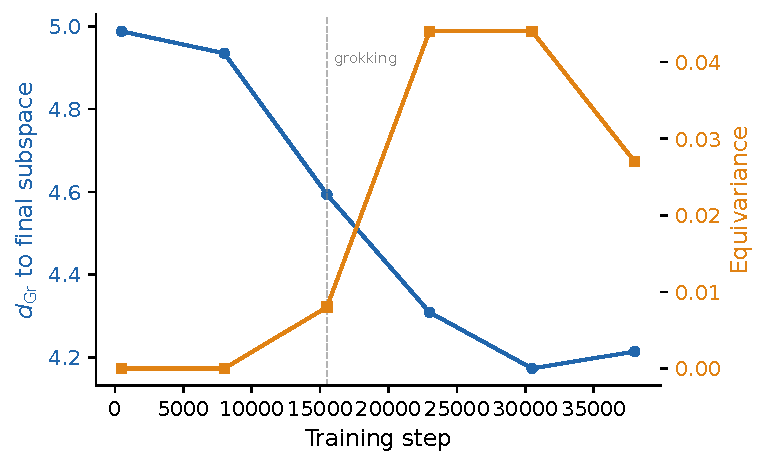
\includegraphics[width=\linewidth]{fig3_trajectory}
\caption{Grassmannian trajectory during grokking for modular
multiplication. The Grassmannian distance $d_{\Gr}$ from the current
DAS subspace to the final (fully grokked) subspace decreases as
equivariance rises. The subspace converges to its final position
during the grokking phase transition (dashed line), confirming that
spectral compression and causal structure emerge simultaneously.}
\label{fig:trajectory}
\end{figure}


\end{document}
